\documentclass{ieeeaccess}

\usepackage{cite}
\usepackage[T1]{fontenc}
\usepackage[utf8]{inputenc}
\usepackage{xcolor}
\usepackage{amsmath,amssymb,amsfonts}
\usepackage{algorithmic}
\usepackage{algorithm}
\usepackage{graphicx}
\usepackage{textcomp}
\usepackage{booktabs,multirow,array,tabularx}
\usepackage{enumitem}
\usepackage{siunitx}
\usepackage[hidelinks,breaklinks]{hyperref}

\graphicspath{{figures/}}

\newcommand{\pp}{\,\text{pp}}

\def\BibTeX{{\rm B\kern-.05em{\sc i\kern-.025em b}\kern-.08em
    T\kern-.1667em\lower.7ex\hbox{E}\kern-.125emX}}
% Items the authors must complete before submission are printed in red brackets.
\xdef\xfigwd{0pt}% lets the class wrap long figure captions
\newcommand{\fillin}[1]{{\color{red}[#1]}}
\newcommand{\doiref}[1]{\href{https://doi.org/#1}{doi: #1}}
\renewcommand{\algorithmicrequire}{\textbf{Input:}}
\renewcommand{\algorithmicensure}{\textbf{Output:}}

\begin{document}
\history{Date of publication xxxx 00, 0000, date of current version xxxx 00, 0000.}
\doi{10.1109/ACCESS.2026.DOI}

\title{Predicting Motor-Imagery BCI Performance from Resting-State EEG with Graph Neural Networks: A Subject-Independent Regression Benchmark}
% ============================================================
% AUTHORS AND AFFILIATIONS
% ============================================================

\author{
\uppercase{S. Krithik Ragav}\authorrefmark{1},
\uppercase{Kamalesh N.}\authorrefmark{2},
\uppercase{Priyankaa S.}\authorrefmark{2},
\uppercase{Dr. Shri Devi S}\authorrefmark{2},
and \uppercase{Dr. Harish Gunasekaran}\authorrefmark{3}
}

\address[1]{Department of Electronics and Communication Engineering, Vellore Institute of Technology, Chennai Campus, Chennai 600127, Tamil Nadu, India (e-mail: krithikragav.s2024@vitstudent.ac.in)}
\address[2]{School of Computer Science and Engineering, Vellore Institute of Technology, Chennai Campus, Chennai 600127, Tamil Nadu, India (e-mail: kamalesh.n2024@vitstudent.ac.in, priyankaa.s2024@vitstudent.ac.in, shridevi.s@vit.ac.in)}
\address[3]{Adjunct Professor, Vellore Institute of Technology, Chennai 600127, Tamil Nadu, India (e-mail: harish.gunasekaran@vit.ac.in)}

\tfootnote{This work was supported in part by the Computational Neuroscience and Neuroengineering Initiative (CNI).}

\corresp{Corresponding author: Dr. Shri Devi S, School of Computer Science and Engineering, Vellore Institute of Technology, Chennai Campus, Chennai 600127, Tamil Nadu, India (e-mail: shridevi.s@vit.ac.in).}

\begin{abstract}
Motor-imagery brain--computer interfaces (MI-BCIs) show large inter-subject performance variability and usually require lengthy user calibration. Earlier work has linked resting-state EEG to MI-BCI performance through correlations, group comparisons, binary high/low screening and deep regression on connectivity indicators. We instead apply message-passing graph neural networks directly to subject-specific electrode graphs for continuous, subject-level prediction under leave-one-subject-out (LOSO) validation. On the 109 participants of the PhysioNet EEG Motor Movement/Imagery Database, relative spectral power (640-D) and weighted phase lag index (wPLI) connectivity graphs from eyes-open and eyes-closed baselines predict the mean of two balanced accuracies (left- vs.\ right-fist and both-fists vs.\ both-feet imagery) from independently cross-validated CSP--LDA decoders (split-half reliability $0.8920$). Scaling, tuning and fitting are fold-internal. A three-layer graph convolutional network (GCN) on sparse alpha-band wPLI graphs reached out-of-fold $r=0.4615$, $R^2=+0.2119$ and $\text{MAE}=10.44$ percentage points (pp); a random forest on spectral features reached $r=0.4328$ and $R^2=+0.1857$. An equal-weight GCN + random forest hybrid gave the highest $r$ ($0.4716$), the highest $R^2$ ($+0.2221$) and the lowest RMSE ($12.90\pp$); ridge ($R^2=-0.0027$) and SVR ($R^2=+0.0749$) were weaker. Subject-level bootstrap intervals, paired model differences, a graph ablation and a subject-level target-permutation test ($p < 0.001$) are reported. Predictions were strongly compressed toward the cohort mean (slope $0.22$), $30.3\%$ of participants had errors above $15\pp$, and design choices were made with access to LOSO results. The study is a subject-independent benchmark, not evidence for clinical use or individual calibration decisions.
\end{abstract}

\begin{keywords}
Brain--computer interfaces, electroencephalography, motor imagery, resting-state EEG, graph neural networks.
\end{keywords}

\titlepgskip=-15pt

\maketitle

% ============================================================
\section{Introduction}
% ============================================================

\PARstart{B}{rain--computer} interfaces (BCIs) provide a direct communication and control channel between the human nervous system and external devices without relying on peripheral muscular pathways~\cite{wolpaw2002,pfurtscheller2001}. Among non-invasive modalities, electroencephalography (EEG) based on motor imagery (MI) is one of the most widely investigated paradigms. During MI, users mentally rehearse movements such as hand opening/closing or foot dorsiflexion, modulating sensorimotor rhythms in the $\mu$ (8--12 Hz) and $\beta$ (13--30 Hz) bands through event-related desynchronization (ERD) and synchronization (ERS)~\cite{pfurtscheller2001,blankertz2008}.

Despite decades of progress in spatial filtering and machine learning~\cite{lotte2018,ang2012,ramoser2000}, a major obstacle to deployment is the pronounced variability of decoding performance across individuals. A substantial fraction of participants (often reported between 15\% and 30\%) show poor control under standard protocols, a phenomenon termed ``BCI illiteracy'' or BCI inefficiency~\cite{blankertz2010,jeunet2016,singh2021}. Conventional MI-BCIs therefore require time-consuming calibration sessions to collect many task trials from each new user, which fatigues participants, increases setup time, and hinders clinical translation.

This motivates the question: \textit{can an individual's expected continuous MI-BCI decoding performance be predicted before task execution from pre-task resting-state EEG?} If so, protocols could in principle be personalized prospectively.

Blankertz \textit{et al.}~\cite{blankertz2010} showed that resting sensorimotor-rhythm power in two Laplacian channels correlated ($r=0.53$) with later BCI feedback accuracy in 80 BCI-naive participants. Wang \textit{et al.}~\cite{wang2022} used relative power, spectral entropy and Lempel--Ziv complexity of resting EEG from 105 participants of the same PhysioNet dataset used here to separate high- from low-performance groups ($85.24\%$ accuracy). Lee \textit{et al.}~\cite{lee2020} applied dynamic causal modeling to resting-state EEG from a public MI dataset and related the effective connectivity from the supplementary motor area to the right dorsolateral prefrontal cortex to MI performance ($r=0.54$ and $r=0.42$ in two sessions). Caicedo-Acosta \textit{et al.}~\cite{caicedo2021} trained deep neural regression models on EEG functional-connectivity indicators under leave-one-out cross-validation on two public databases (150 users in total). Resting-state prediction of MI-BCI performance, including continuous and connectivity-based prediction under held-out evaluation, is therefore established, and we do not claim it as new. What remains less explored in this literature, and what this paper targets, is the following:

\begin{enumerate}[leftmargin=*]
    \item \textbf{Dichotomization of continuous performance:} several studies binarize decoding accuracy into high and low performers, discarding fine-grained variation.
    \item \textbf{Evaluation protocol:} many analyses report in-sample correlations, group comparisons or epoch-level random splits, which do not measure prediction for a subject that was fully held out of scaling, tuning and fitting.
    \item \textbf{Graph structure not learned:} connectivity enters either as a few hand-selected edges or as a vectorized matrix, whereas message-passing graph neural networks, which use the electrode graph directly, have been applied to trial-wise classification but, to our knowledge, not to subject-level prediction of MI-BCI performance from resting EEG. Connectivity-derived indicators fed to dense regression networks~\cite{caicedo2021} are the closest prior approach.
    \item \textbf{Target reliability and error structure:} the repeatability of the performance target and the structure of prediction errors (shrinkage toward the mean, error by performance level) are rarely quantified.
\end{enumerate}

We address these gaps on the 109-subject PhysioNet EEG Motor Movement/Imagery Database (EEGMMIDB)~\cite{goldberger2000,physionet2009}. Cohort size is not a differentiator: Wang \textit{et al.}~\cite{wang2022} analyzed 105 subjects of the same database, and Caicedo-Acosta \textit{et al.}~\cite{caicedo2021} also used it. Using eyes-open and eyes-closed baselines, we evaluate continuous subject-level regression under LOSO cross-validation with fold-internal tuning. We compare relative power spectral density (PSD) and wPLI~\cite{vinck2011} connectivity graphs processed by graph convolutional networks (GCNs)~\cite{kipf2017}, a residual dual-band GCN, random forests, linear and kernel baselines, and ensembles.

The contributions are:

\begin{enumerate}[leftmargin=*]
    \item \textbf{Message-passing GNN regression of MI-BCI performance from resting EEG:} the main contribution is to predict a continuous MI-BCI performance score from subject-specific resting-state electrode graphs (spectral node features, sparse wPLI edges) with graph convolutional networks, with every prediction made for a subject fully excluded from scaling, tuning and fitting. Continuous prediction from connectivity indicators has been done before~\cite{caicedo2021}; the new element is the graph-learning formulation and its evaluation against ablations and a permutation reference.
    \item \textbf{Sparse connectivity-graph model:} a graph combining 10-D multi-condition spectral node features with alpha-band wPLI edges, processed by a compact 3-layer GCN that achieves higher point estimates than ridge and RBF-SVR baselines ($R^2=+0.2119$, $r=0.4615$).
    \item \textbf{Spectral--graph hybrid:} an equal-weight GCN + random forest ensemble with the highest Pearson $r$ ($0.4716$), $R^2$ ($+0.2221$) and lowest RMSE ($12.90\pp$) among the evaluated models; the lowest MAE ($10.40\pp$) was achieved by the GCN Ensemble.
    \item \textbf{Evidence for or against the graph:} subject-level bootstrap intervals and paired differences for all models, a graph ablation (vectorized wPLI, identity and shuffled adjacency, node-feature-only model) and a subject-level target-permutation test.
    \item \textbf{Reliable target and error analysis:} a composite of two independently decoded imagery tasks with split-half reliability $\mathrm{SB}=0.8920$, together with quantification of regression-to-the-mean shrinkage, quartile-dependent error against a mean baseline, and the distribution of absolute errors.
\end{enumerate}

% ============================================================
\section{Related Work and Research Gap}
% ============================================================

\subsection{Inter-Subject Variability and BCI Inefficiency}

Inter-subject variability in MI-BCI is attributed to anatomical differences, baseline sensorimotor rhythm power, psychological factors such as attention and spatial visualization ability, and neuroplastic adaptability~\cite{jeunet2016,blankertz2010,lotte2018}. Common Spatial Pattern (CSP)~\cite{ramoser2000} and Filter Bank CSP (FBCSP)~\cite{ang2012} learn spatial filters that contrast class variances, but degrade when a user does not produce clear, focal ERD/ERS. Predicting this variability from pre-task neurophysiology is therefore a central research priority~\cite{singh2021}.

\subsection{Resting-State Electrophysiology as a Predictor}

Resting-state EEG reflects intrinsic oscillatory dynamics~\cite{pfurtscheller2001}. Blankertz \textit{et al.}~\cite{blankertz2010} identified resting $\mu$-rhythm amplitude as a predictor, reasoning that higher baseline power leaves a larger dynamic range for ERD during imagery. Later work used spectral entropy~\cite{zhang2015entropy}, Lempel--Ziv complexity~\cite{wang2022} and microstate durations~\cite{cui2023}, and related resting-state network measures~\cite{zhang2015network} and dynamic-causal-modeling effective connectivity~\cite{lee2020} to MI performance. These studies confirmed that resting activity relates to BCI performance, but they relied on correlations, group comparisons or binary screening, or used modest cohorts; to our knowledge none applied message-passing graph neural networks to the electrode graph for this prediction problem. The closest work~\cite{caicedo2021} fed connectivity-derived indicators to deep dense regression networks with leave-one-out validation. Reviews of MI-EEG decoding also stress dataset heterogeneity and inconsistent validation protocols that hinder comparison across studies~\cite{khademi2023,wang2024survey,saibene2024,saibene2023wearable}. Table~\ref{tab:prior_comparison} places the present subject-independent regression benchmark in relation to representative resting-state studies. This motivates a narrow, auditable question: is a resting-state representation associated with an independently measured continuous target when the participant, rather than the epoch, is held out?

\subsection{Functional Connectivity and Graph Neural Networks}

Sensorimotor control relies on coordinated communication across distributed fronto-parietal and inter-hemispheric networks~\cite{hamedi2016,zhang2015network}. Spectral power captures local synchronization but not phase coupling between distant regions. The weighted phase lag index (wPLI)~\cite{vinck2011} reduces sensitivity to zero-lag coupling from volume conduction by weighting phase differences with the magnitude of the imaginary cross-spectrum.

Graph neural networks generalize convolution to non-Euclidean domains and suit EEG, where electrodes are nodes and functional connectivity forms edges~\cite{kipf2017,velickovic2018,hamilton2017}. CNN and graph models have mostly been applied to trial-wise task classification~\cite{schirrmeister2017,lawhern2018,sun2023graph,xue2024,shi2024}. The present study differs in prediction unit and target: it estimates a subject-level decoding-performance summary from separate resting recordings, so classification accuracies of graph-based MI decoders are not comparable to the regression metrics reported here.

\begin{table*}[!t]
\caption{Comparison With Representative Resting-State or Pre-Task MI-BCI Performance Studies}
\label{tab:prior_comparison}
\centering
\scriptsize
\begin{tabularx}{\textwidth}{p{2.4cm}p{0.7cm}p{2.6cm}p{2.3cm}p{2.2cm}X}
\toprule
\textbf{Study} & \textbf{$N$} & \textbf{Input Modality} & \textbf{Target Formulation} & \textbf{Evaluation Scheme} & \textbf{Relationship to Present Work}\\
\midrule
Blankertz \textit{et al.}~\cite{blankertz2010} & 80 & 2-min eyes-open resting EEG (2 Laplacian channels) & Continuous SMR-BCI feedback accuracy & Correlation analysis & Established feasibility of resting SMR power predictors; two channels, no graph topology, no LOSO regression.\\
Bamdadian \textit{et al.}~\cite{bamdadian2014} & 17 & Pre-cue spectral rhythms across regions & MI classification performance & Group-level correlation & Pre-cue spectral relevance in a small cohort; no subject-independent out-of-sample testing.\\
Zhang \textit{et al.}~\cite{zhang2015entropy} & 40/26 & Eyes-open/closed resting EEG (spectral entropy) & Inter-session SMR-BCI performance & Session-wise prediction & Resting complexity predicts cross-session stability; scalar entropy rather than graph learning.\\
Caicedo-Acosta \textit{et al.}~\cite{caicedo2021} & 50 & Pre-cue / short-window functional connectivity indicators, public MI databases & Continuous MI skill / inefficiency measures & Leave-one-out CV with Monte Carlo dropout & Closest prior continuous regression; dense network on connectivity-derived indicators, not message passing on the electrode graph; reported $R^2$ is not directly comparable (different target and pipeline).\\
Lee \textit{et al.}~\cite{lee2020} & 54 & Resting-state EEG effective connectivity (dynamic causal modeling) & MI performance, high/low groups and continuous & Group comparison and correlation ($r=0.54$, $0.42$) & Hand-selected effective-connectivity predictor on a different public MI dataset; no learned graph model, no LOSO regression.\\
Wang \textit{et al.}~\cite{wang2022} & 105 & Eyes-open/closed resting EEG (PSD, PSE, LZC), same EEGMMIDB dataset & Binary high/low MI screening & Stratified cross-validation & 85.24\% binary screening accuracy with the best feature (PSE); the present work uses continuous regression, graph models and LOSO.\\
Cui \textit{et al.}~\cite{cui2023} & 28 & Resting EEG microstate parameters & Continuous MI classification accuracy & 10-fold cross-validation & Microstate dynamics in 28 subjects; the present work uses 109 subjects and graph connectivity.\\
\textbf{Present Work} & \textbf{109} & \textbf{64 channels: 10-D PSD node features + wPLI graphs} & \textbf{Continuous composite CSP--LDA accuracy ($0.5[\text{T2}+\text{T4}]$)} & \textbf{Strict 109-fold LOSO with fold-internal tuning} & \textbf{Continuous regression with graph models under LOSO; spectral power and wPLI graphs via GCN and hybrid ensemble ($R^2=+0.2221$).}\\
\bottomrule
\end{tabularx}
\end{table*}

% ============================================================
\section{Dataset and Target Definition}
% ============================================================

\subsection{PhysioNet EEGMMIDB Cohort}

Experiments use the public PhysioNet EEGMMIDB~\cite{goldberger2000,schalk2004,physionet2009}: 64-channel EEG (10--10 montage) from 109 healthy volunteers, sampled at 160 Hz. Each participant completed 14 runs:

\begin{itemize}[leftmargin=*]
    \item \textbf{Run 1 (R01):} baseline, eyes open (60 s).
    \item \textbf{Run 2 (R02):} baseline, eyes closed (60 s).
    \item \textbf{Runs 3, 7, 11:} motor execution, left or right fist.
    \item \textbf{Runs 4, 8, 12 (Task 2):} motor imagery, left fist vs.\ right fist.
    \item \textbf{Runs 5, 9, 13:} motor execution, both fists or both feet.
    \item \textbf{Runs 6, 10, 14 (Task 4):} motor imagery, both fists vs.\ both feet.
\end{itemize}

Every participant completed both baselines ($109\times2=218$ resting recordings). The dataset audit identified three recordings (S088, S092, S100) as natively sampled at 128 Hz; these recordings bypass the 160-to-128-Hz resampling step. Subject S089, whose annotations are documented as inconsistent in literature, was audited and handled through a verified run mapping. No participant was excluded, so the analytic cohort is $N=109$.

\subsection{Recording Separation and Analytical Roles}

To prevent leakage, recordings are partitioned into non-overlapping branches (Table~\ref{tab:data_roles}). Baseline runs (R01, R02) serve only as predictor inputs $\mathbf{x}_i$; imagery runs (R04, R06, R08, R10, R12, R14) serve only to construct the target $y_i$.

\begin{table}[!t]
\caption{Analytical Roles of EEG Recordings}
\label{tab:data_roles}
\centering
\small
\begin{tabular}{p{1.35cm}p{1.8cm}p{3.0cm}}
\toprule
\textbf{Branch} & \textbf{Runs Used} & \textbf{Methodological Purpose}\\
\midrule
Predictor Input & R01 (EO), R02 (EC) & Spectral PSD (640-D) and wPLI connectivity graphs ($64\times64$).\\
Target Source & R04, R08, R12 (Task 2) & CSP--LDA decoding of left- vs.\ right-fist imagery.\\
& R06, R10, R14 (Task 4) & CSP--LDA decoding of both-fists vs.\ both-feet imagery.\\
\bottomrule
\end{tabular}
\end{table}

\subsection{Continuous Target Construction}

The target is an estimated decoder-performance measure: balanced accuracy obtained from task EEG with a leakage-safe 5-fold cross-validated CSP--LDA pipeline~\cite{ramoser2000,ang2012}, in which CSP filters and the (shrinkage-regularized) LDA classifier are fitted on training folds only.

For two-class covariance matrices $C_1$, $C_2$, spatial filters $w$ solve
\begin{equation}
C_1 w = \lambda (C_1 + C_2) w .
\end{equation}
Projected signals $z_k(t)=w_k^T x(t)$ are converted to normalized log-variance features $f_k=\log\bigl(\operatorname{var}(z_k)/\sum_j \operatorname{var}(z_j)\bigr)$ and classified with LDA. Balanced accuracy is
\begin{equation}
\mathrm{BA} = \frac{1}{2} \left( \frac{TP}{TP + FN} + \frac{TN}{TN + FP} \right).
\end{equation}

\subsection{Composite Target and Target Reliability}

To reduce the trial-to-trial variance of any single task, the target is the task-coherent composite
\begin{equation}
y_i = \frac{1}{2} \left( \mathrm{BA}_{\text{Task 2}, i} + \mathrm{BA}_{\text{Task 4}, i} \right) \in [0, 1].
\end{equation}
It spans a lateralized upper-limb contrast (left vs.\ right fist) and a bilateral-hand vs.\ lower-limb contrast (both fists vs.\ both feet).

Single-task targets show moderate split-half reliability ($\mathrm{SB}=0.7908$ for Task 2, $0.8586$ for Task 4; $\mathrm{ICC}(3,1)=0.6358$ and $0.6821$). The composite reaches $\mathrm{SB}=0.8920$. This reported Spearman--Brown split-half reliability reflects internal consistency across trial partitions within the single recording session; it is not a longitudinal test--retest reliability estimate. Task 2 and Task 4 accuracies correlate across subjects ($r=0.5356$, 95\% CI $[0.3865, 0.6575]$, $p=1.96\times10^{-9}$; Spearman $\rho=0.4886$; disattenuated $r = 0.6500$, i.e., about $42.3\%$ shared true variance ($r_{\mathrm{dis}} = 0.5356 / \sqrt{0.7908 \times 0.8586} = 0.6500$), supporting cross-task construct validity (Fig.~\ref{fig:target_reliability}). The composite ranges from $34.26\%$ to $98.91\%$ (mean $63.86\%$, SD $14.69\%$; quartile boundaries $53.7\%$, $61.3\%$, $72.7\%$).

\begin{figure*}[!t]
\centering
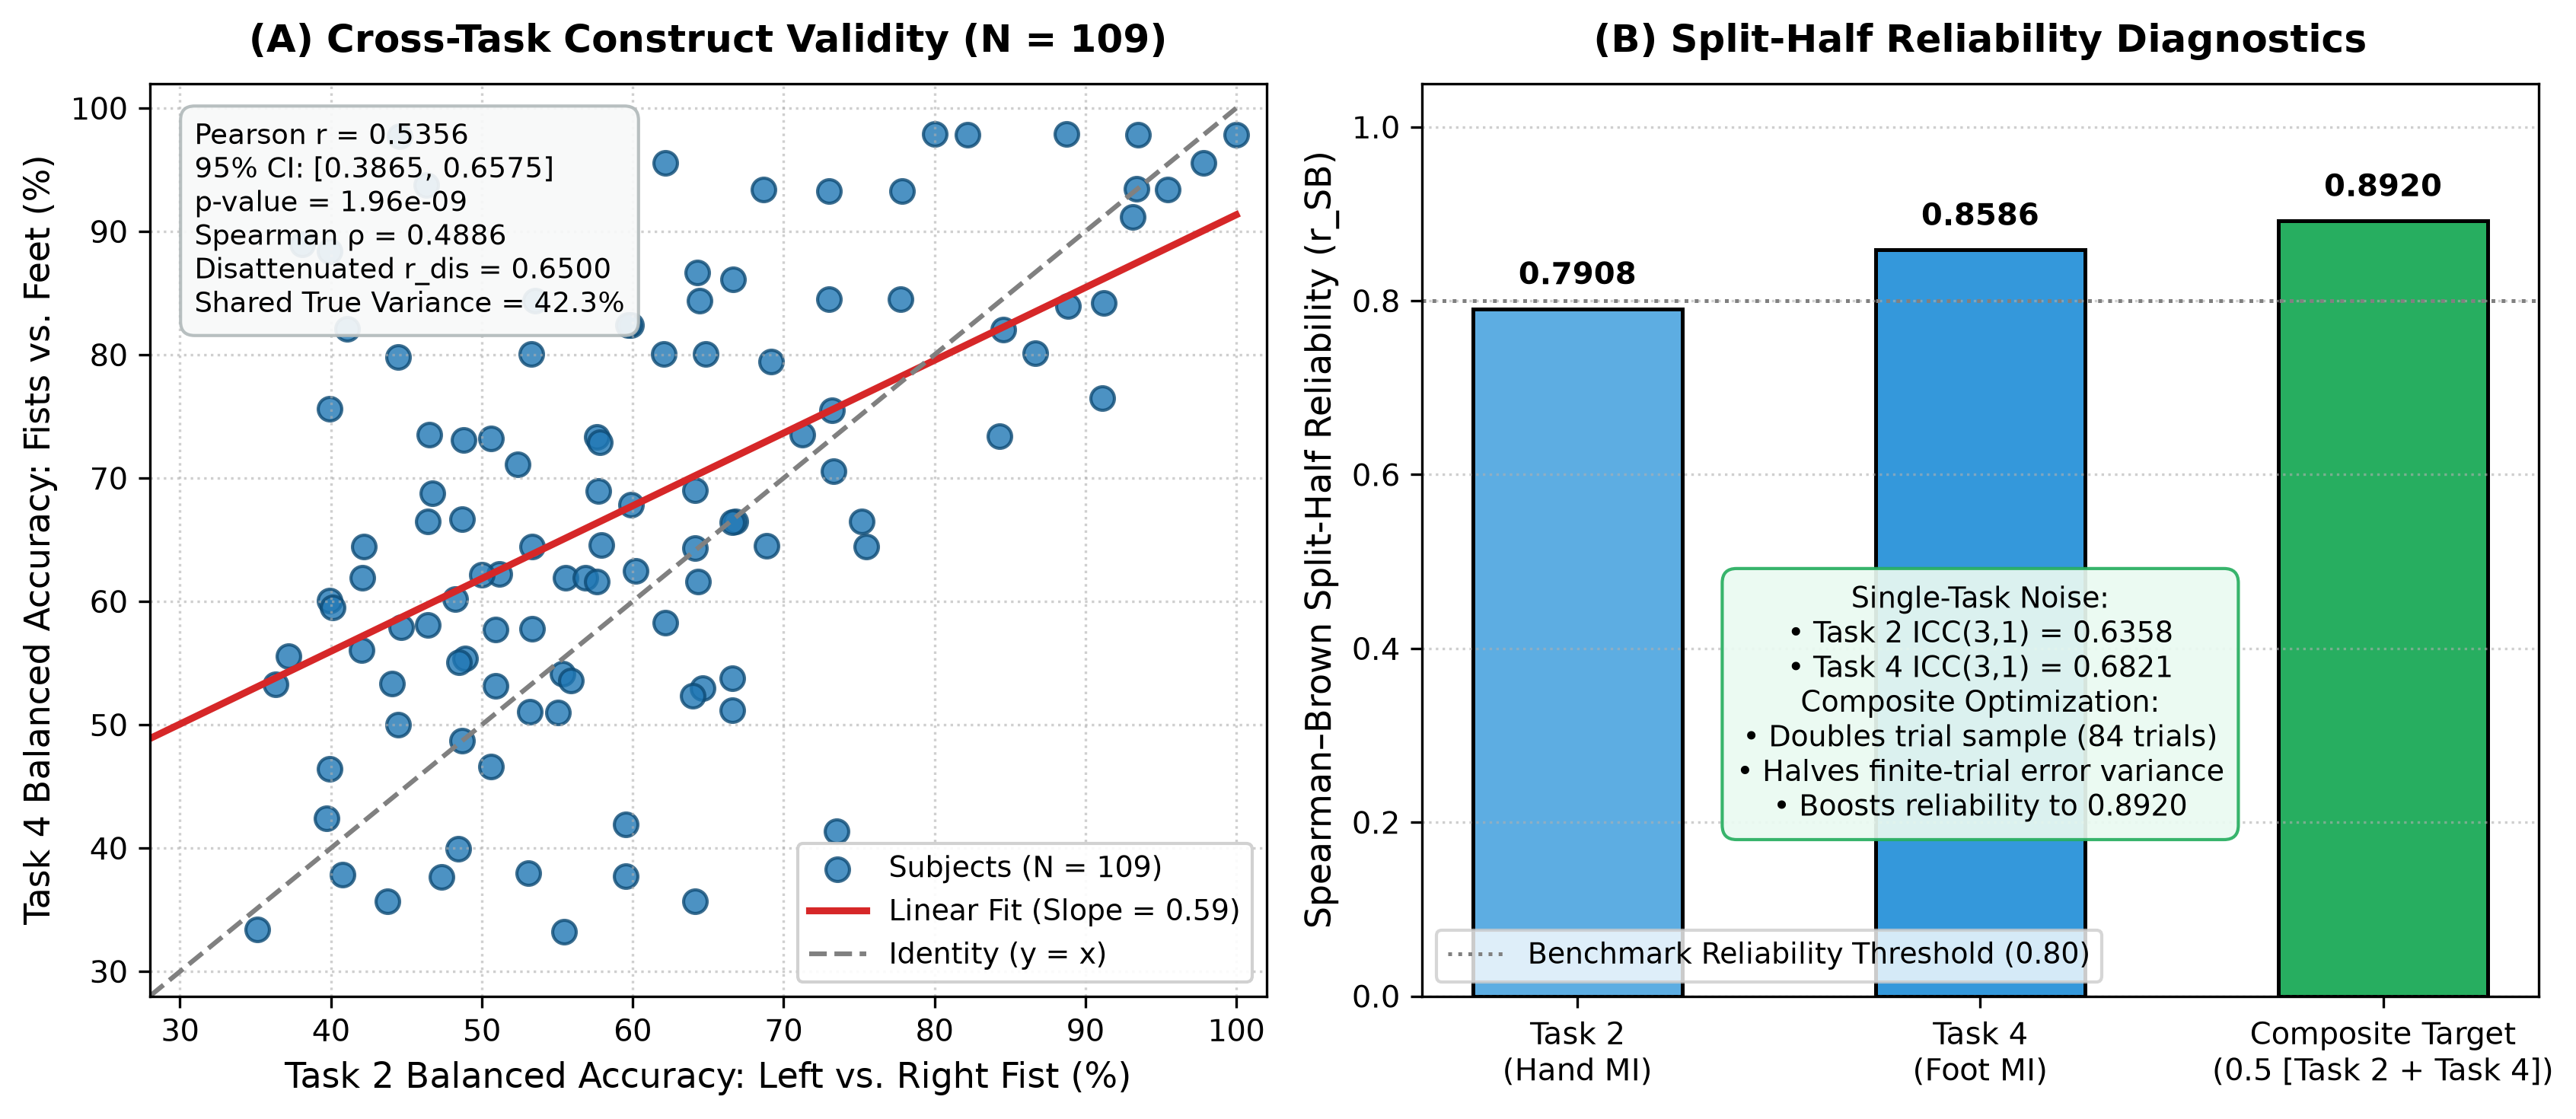
\includegraphics[width=\textwidth]{figure2_target_validity_reliability.png}
\caption{Construct validity and split-half reliability of the MI decoding targets ($N=109$). (A) Cross-task association between Task 2 (left vs.\ right fist) and Task 4 (both fists vs.\ both feet) balanced accuracy; the dashed line is $y=x$ and the solid line is the least-squares fit. (B) Spearman--Brown split-half reliability of Task 2, Task 4 and the composite target; the dotted line marks the conventional 0.80 level.}
\label{fig:target_reliability}
\end{figure*}

\subsection{Meaning and Limits of the Composite Target}

The composite represents performance across two related but non-identical imagery tasks under this specific CSP--LDA decoder and these two tasks; it is not a general or decoder-independent measure of intrinsic BCI aptitude. Averaging the two balanced accuracies with equal weight is transparent and avoids fitting a target combination against the resting-state predictors. It does not imply that the tasks are interchangeable, nor does it identify a latent aptitude. Balanced accuracy is less sensitive to class prevalence than accuracy, but remains subject to finite-trial uncertainty, signal quality, artifact rejection and CSP stability. Within-participant cross-validation reduces optimism but does not make the target error-free. The split-half result shows that the composite is more repeatable under the chosen trial partition than either component; it is not a test--retest estimate and does not make the target an immutable trait. A non-perfect cross-task correlation is expected because the tasks differ in imagery content, cortical recruitment and difficulty. Alternative, multivariate latent-variable targets should be pre-specified and validated independently to avoid tuning the target to the predictors.

% ============================================================
\section{Resting-State Preprocessing and Feature Extraction}
% ============================================================

\subsection{Standardized Preprocessing Pipeline}

Resting recordings pass through a frozen, automated pipeline:

\begin{enumerate}[leftmargin=*]
    \item \textbf{Notch filtering:} 60-Hz notch for US line interference (second-order Butterworth, $Q = 30$), applied first, before the band-pass stage.
    \item \textbf{Band-pass filtering:} zero-phase FIR, 1--40 Hz (Hamming window). The notch filter was applied prior to band-pass filtering to suppress high-amplitude powerline harmonics and eliminate potential spectral leakage into sub-harmonics during anti-aliasing decimation; it is retained in the frozen pipeline to ensure exact numerical reproducibility.
    \item \textbf{Resampling:} 160-Hz recordings are polyphase-resampled (anti-aliased) to 128 Hz, whose Nyquist frequency of 64 Hz bounds the 40-Hz upper band edge (native 128-Hz recordings bypass this step).
    \item \textbf{Re-referencing:} common average reference (CAR) over all 64 electrodes.
    \item \textbf{Epoching and QC:} 2-s non-overlapping epochs (30 per 60-s run); epochs exceeding $\pm100\,\mu\text{V}$ are rejected. FastICA ($n=20$ components) was used for artifact auditing only; ICA-cleaned signals are not part of the final pipeline. Across the 218 resting recordings, a mean of $29.98$ epochs per recording was retained (minimum $29$, maximum 30), with zero epochs rejected by the $\pm100\,\mu\text{V}$ criterion ($0.0\%$ rejection).
\end{enumerate}

\subsection{Relative Power Spectral Density}

PSD $P_c(f)$ is estimated per channel with Welch's method (1-s Hamming windows, 50\% overlap)~\cite{welch1967}. Band power is
\begin{equation}
P_{c,b} = \int_{f_b^{\mathrm{L}}}^{f_b^{\mathrm{H}}} P_c(f)\, df
\end{equation}
for $\delta$ (1--4 Hz), $\theta$ (4--8 Hz), $\alpha$ (8--13 Hz), $\beta$ (13--30 Hz) and $\gamma$ (30--40 Hz) (the wPLI graphs use $\alpha=8$--$12$~Hz; see Sec.~IV-C), and relative power is
\begin{equation}
R_{c,b} = \frac{P_{c,b}}{\sum_{k \in \mathcal{B}} P_{c,k}} .
\end{equation}
Over 64 channels, 5 bands and 2 conditions (EO, EC) this yields $\mathbf{x}_i\in\mathbb{R}^{640}$. Because the five relative powers of a channel/condition sum to one, the vector is compositional (128 linear constraints), which matters for linear models such as ridge regression.

\subsection{Weighted Phase Lag Index Connectivity}

Connectivity is estimated separately for each retained 2-s epoch of both R01 (eyes-open) and R02 (eyes-closed) recordings using a fourth-order zero-phase Butterworth bandpass filter (8--13~Hz for $\alpha$) and analytic Hilbert transform; the imaginary cross-product $\operatorname{Im}(S_{xy}(t))$ is averaged across all time samples of retained epochs to compute condition-wise wPLI matrices, which are then combined as the unweighted arithmetic mean $W_{\text{rest}} = 0.5 (W_{\text{R01}} + W_{\text{R02}})$~\cite{vinck2011}:
\begin{equation}
\mathrm{wPLI}_{xy} = \frac{\left| \sum_{t} \operatorname{Im}(S_{xy}(t)) \right|}{\sum_{t} \left| \operatorname{Im}(S_{xy}(t)) \right|} .
\end{equation}
Because wPLI uses the imaginary cross-spectrum, it is less sensitive to instantaneous volume conduction. It does not guarantee source-level specificity; edges are statistical connectivity estimates, not anatomical connections. Matrices $C\in\mathbb{R}^{64\times64}$ are computed for the alpha (8--12 Hz) and beta (13--30 Hz) bands; the alpha band for wPLI was deliberately restricted to 8--12~Hz (classic sensorimotor $\mu$/alpha range) to prevent phase-estimation instability near the 13-Hz beta boundary, whereas broad-band spectral PSD integration in Sec.~IV-B retained the standard 8--13~Hz band.

\subsection{Subject-Specific Graph Representation}

Each subject is an undirected graph $G=(V,E,W)$ with
\begin{itemize}[leftmargin=*]
    \item \textbf{Nodes:} 64 electrodes.
    \item \textbf{Node features} $X\in\mathbb{R}^{64\times10}$: the 5-band relative PSD of R01 and R02 at each electrode.
    \item \textbf{Edges/adjacency:} the subject-specific alpha-band wPLI matrix ($64\times64$) sparsified to its top 15\% of edges ($\approx 302$ of 2,016 pairs), with degree-1 protection so that no node is isolated. Edges are ranked by wPLI value over the 2,016 upper-triangular pairs of the symmetric matrix (diagonal entries excluded), and the top $\lfloor0.15\times2016\rfloor=302$ are retained. In the event of tied wPLI values, ties are resolved deterministically by ascending channel index order. Degree-1 protection connects any node with zero retained edges to its single highest-wPLI partner. This sparsification is a within-subject deterministic rule and therefore does not require statistics from other subjects.
\end{itemize}

% ============================================================
\section{Complete Experimental Pipeline}
% ============================================================

\begin{figure*}[!t]
\centering
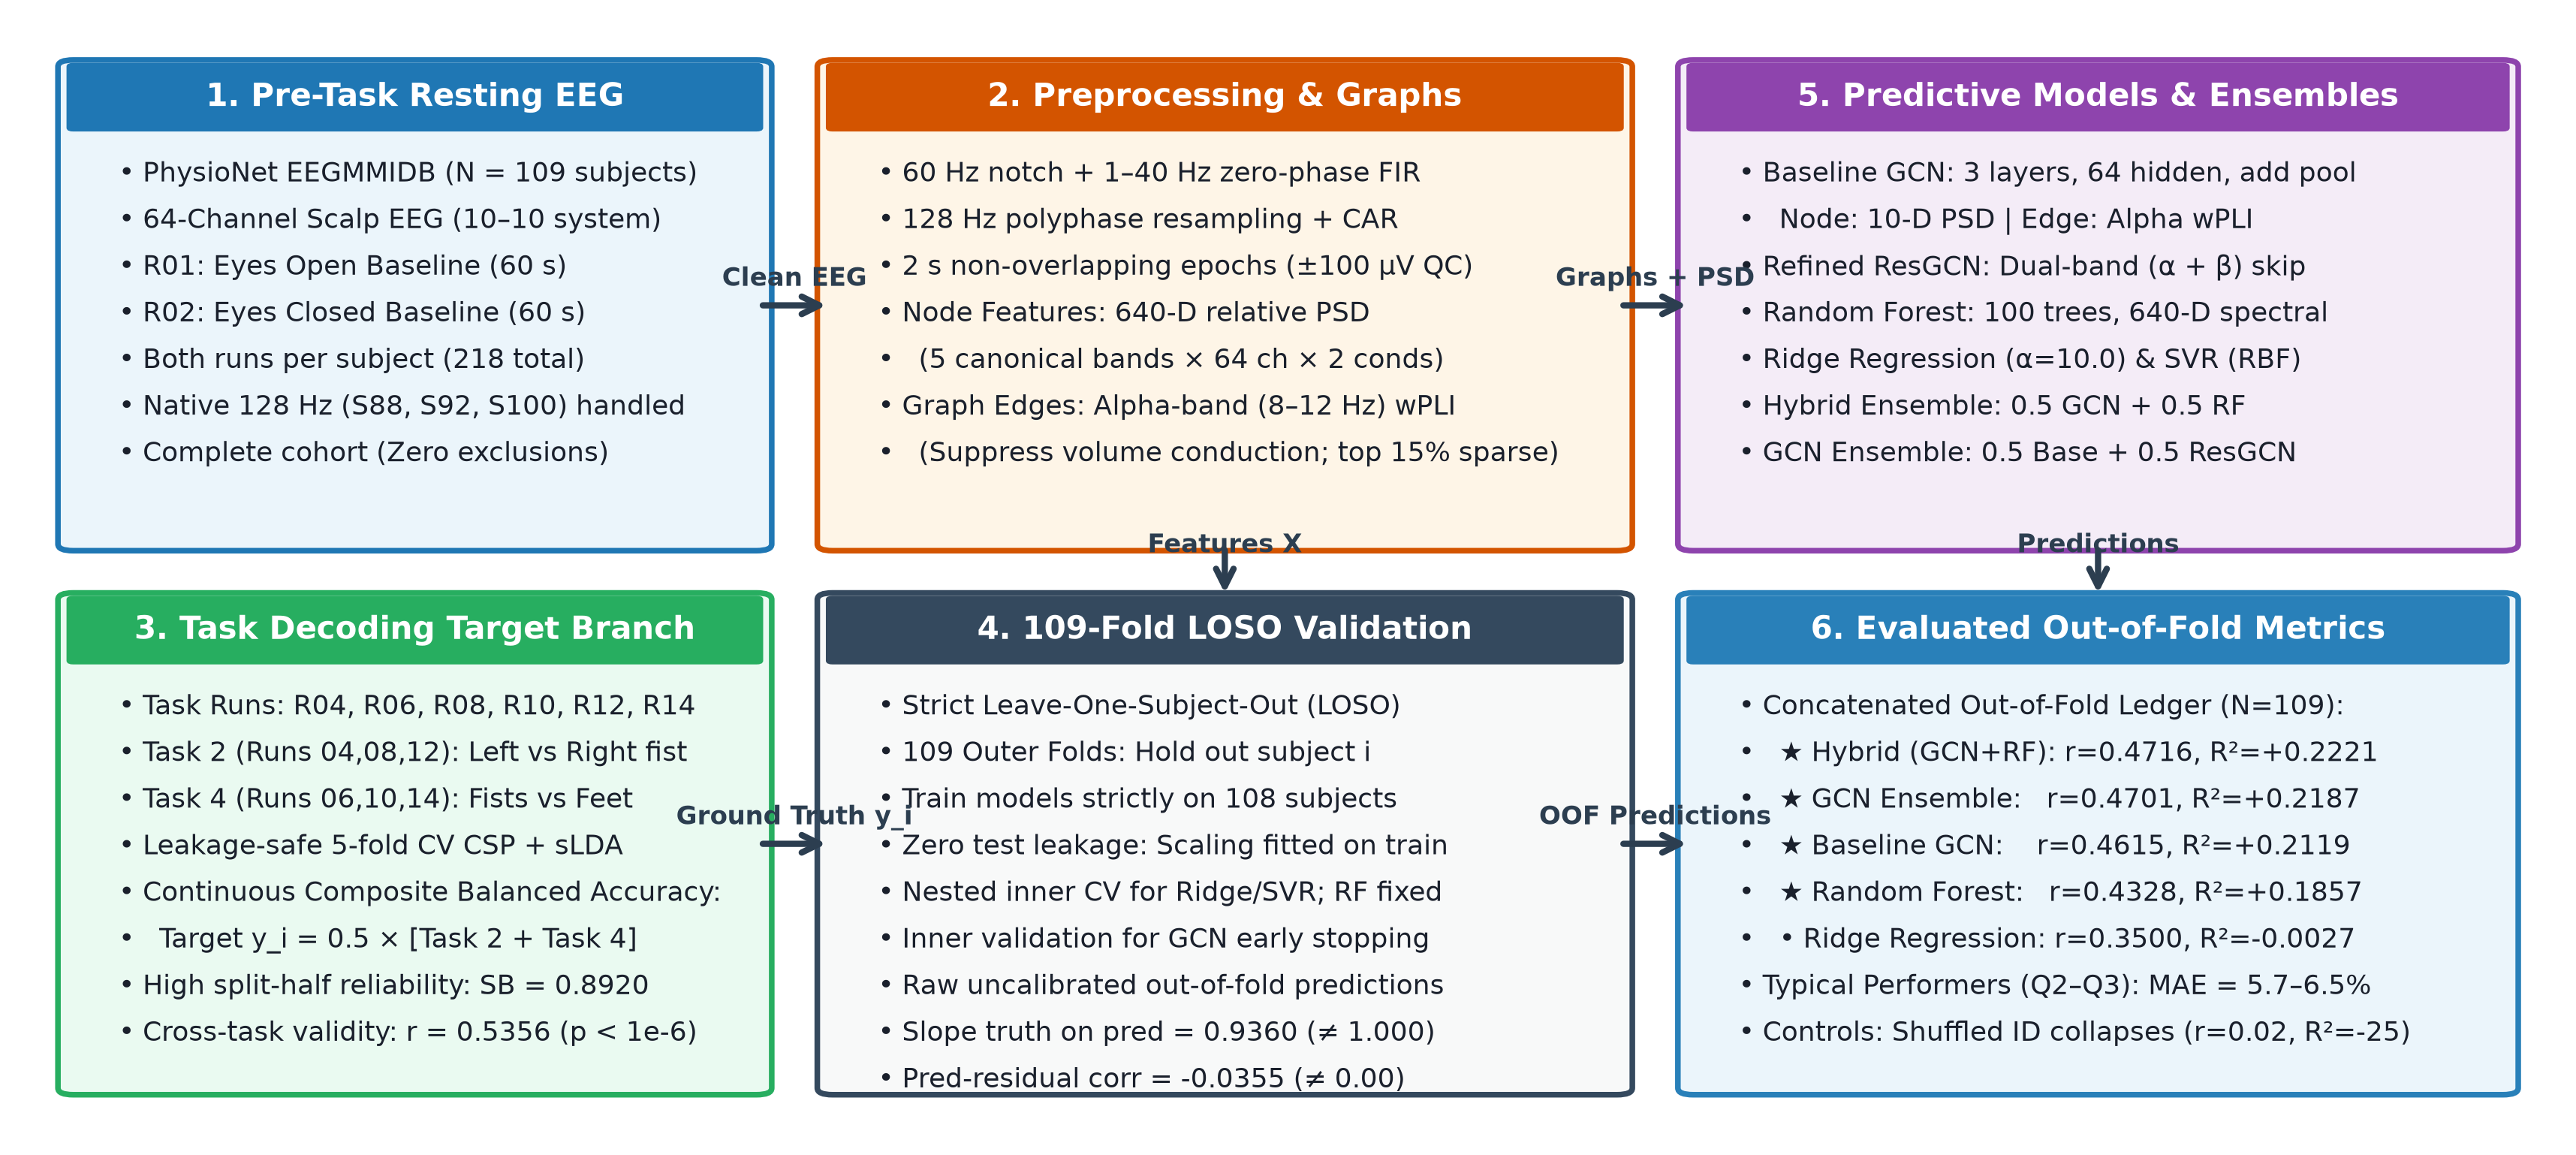
\includegraphics[width=\textwidth]{Fig2_Framework.png}
\caption{Overall framework. (1) Pre-task resting EEG (R01, R02) is processed for each of the 109 subjects. (2) Preprocessing yields 640-D relative spectral features and subject-specific sparse alpha-wPLI graphs. (3) An independent target branch applies leakage-safe 5-fold CSP--LDA decoding to Task 2 and Task 4 and forms the composite target. (4) Strict 109-fold LOSO validation keeps scaling, tuning, fitting, and stopping inside the training subjects. (5) Predictive models and fixed-weight ensembles are evaluated on the concatenated out-of-fold ledger. Panel 6 repeats headline results for orientation; Table~\ref{tab:model_comparison} gives the authoritative values.}
\label{fig:complete_pipeline}
\end{figure*}

The workflow (Fig.~\ref{fig:complete_pipeline}) has six compartmentalized stages; Table~\ref{tab:method_summary} summarizes the corresponding inputs, outputs, and methodological purposes:

\begin{enumerate}[leftmargin=*]
    \item \textbf{Resting EEG ingestion:} R01/R02 baselines are separated from task runs R04--R14 upon ingestion; the subject is the experimental unit.
    \item \textbf{Preprocessing and graphs:} filtering, resampling, CAR, epoch rejection, Welch PSD (640-D) and wPLI graph construction.
    \item \textbf{Target branch:} 5-fold CSP--LDA decoding of Task 2 and Task 4, giving $y_i\in[0,1]$.
    \item \textbf{Strict 109-fold LOSO validation:} in fold $i$, scaling, hyperparameter selection and fitting use only $\mathcal{D}^{(i)}_{\text{train}}=\{(\mathbf{x}_j,y_j) : j\neq i\}$.
    \item \textbf{Models and ensembles:} GCN, ResGCN, random forest, ridge, SVR and the hybrids (Sec.~\ref{sec:models}).
    \item \textbf{Out-of-fold evaluation:} predictions are concatenated into $\hat{\mathbf{y}}_{\text{OOF}}=[\hat y_1,\dots,\hat y_{109}]^T$ and all headline metrics are computed on this vector only.
\end{enumerate}

% ============================================================
\section{Leakage Control and LOSO Protocol}
% ============================================================

Figure~\ref{fig:loso_protocol} summarizes the LOSO protocol. Four leakage pathways were controlled:

\begin{itemize}[leftmargin=*]
    \item \textbf{Subject overlap:} strict LOSO partitioning; no epoch of the test subject enters training.
    \item \textbf{Preprocessing/normalization:} across-subject standardization parameters $\mu_{\text{train}},\sigma_{\text{train}}$ are fitted on the 108 training subjects and then applied to the held-out subject. Subject-specific graph construction uses only the corresponding subject's resting EEG and does not use other subjects.
    \item \textbf{Target--feature isolation:} $y_i$ comes only from task runs (R04--R14); $\mathbf{x}_i$ comes only from baselines (R01, R02).
    \item \textbf{Hyperparameter and stopping selection:} Ridge $\alpha$ and SVR $C$/$\epsilon$ are the only hyperparameters tuned by nested 5-fold cross-validation inside the 108 training subjects. The random-forest configuration ($T=100, m_{\text{try}}=\lfloor\sqrt{640}\rfloor=25$) is fixed a priori (Sec.~\ref{sec:models}), and the GCN uses an inner validation split of the training pool for early stopping only. The held-out subject's target is never used for tuning, stopping, or ensemble weights; the hybrid weights are fixed a priori at $0.5/0.5$.
\end{itemize}

All reported metrics are raw out-of-fold predictions without post-hoc linear recalibration on test labels. Descriptive diagnostics of the Primary GCN are a regression slope of the observed target on predictions of $0.9360$ (identity would be $1.0000$) and a prediction--residual correlation of $-0.0355$. These diagnostics are descriptive; absence of recalibration is established by the procedure and the prediction ledger, not by the slope.

\begin{figure*}[!t]
\centering
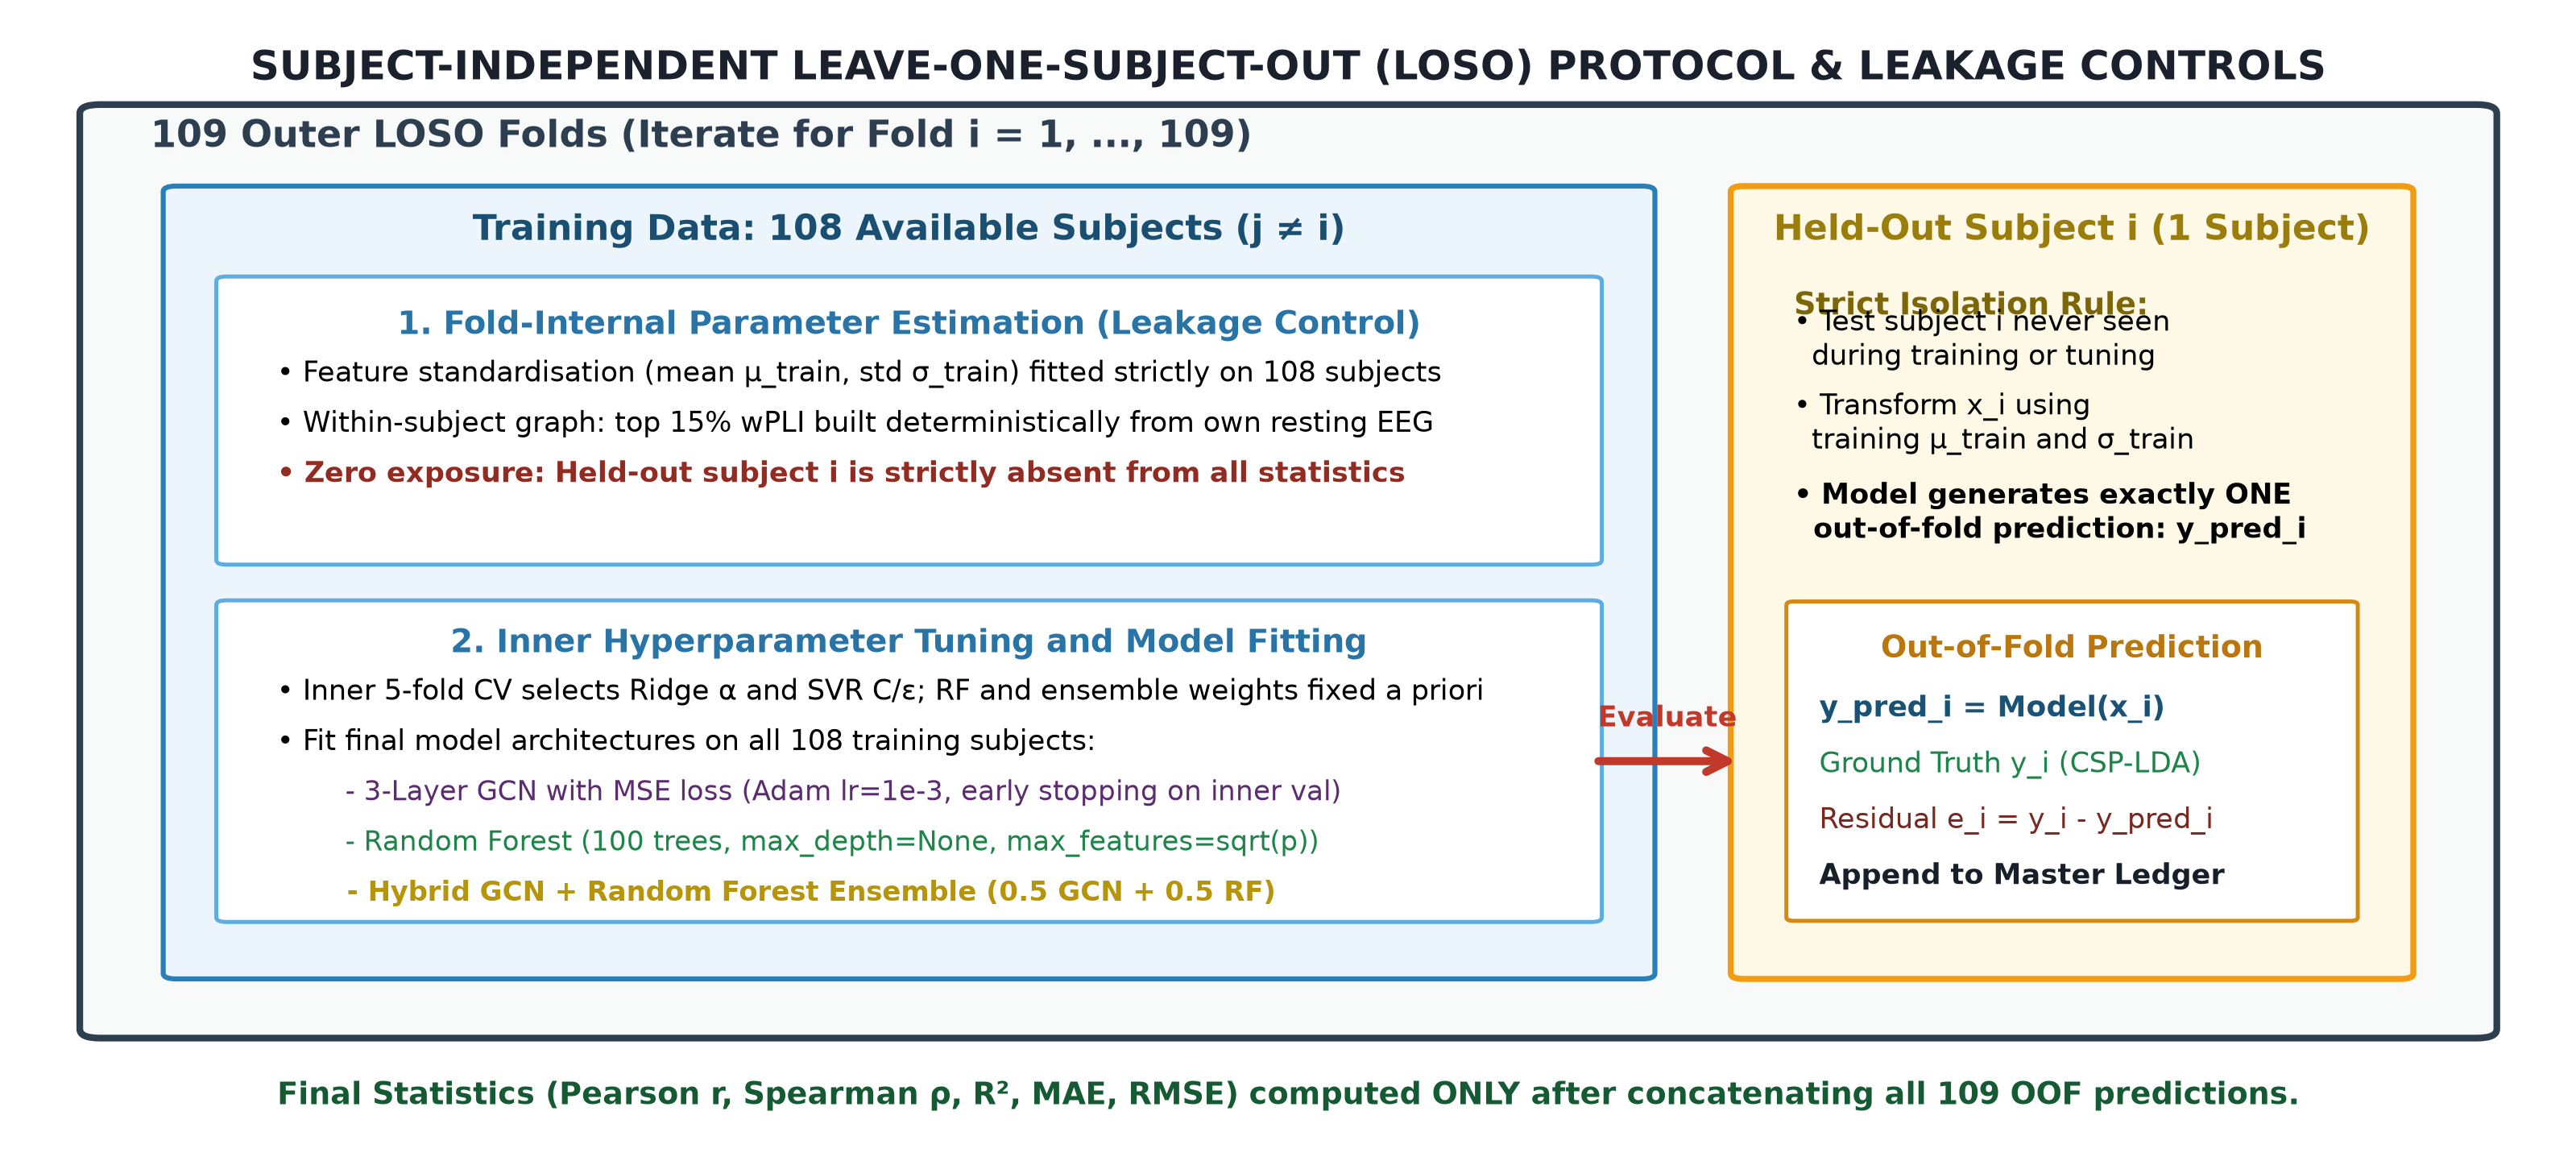
\includegraphics[width=\textwidth]{Fig3_LOSO_Protocol.png}
\caption{Subject-independent LOSO protocol and leakage controls. In each of the 109 outer folds, feature standardization and learned model parameters use only the 108 training subjects; subject-specific graphs are constructed from each subject's own resting EEG, ridge and SVR hyperparameters are selected by nested 5-fold inner cross-validation, GCN early stopping uses an inner validation split, the random forest and ensemble weights are fixed a priori, and the held-out subject receives exactly one out-of-fold prediction that is appended to the ledger.}
\label{fig:loso_protocol}
\end{figure*}


% ============================================================
\section{Methodology Summary}
% ============================================================

The analysis comprised six stages: separation of resting and task recordings (Sec.~III), preprocessing and feature or graph construction (Sec.~IV), target estimation by independently cross-validated CSP--LDA decoders (Sec.~III-C), model fitting and tuning inside each LOSO fold (Secs.~V--VI and VIII), and evaluation on the 109 concatenated out-of-fold predictions (Sec.~IX). The leakage controls are described once in Sec.~VI and are not repeated here. Table~\ref{tab:method_summary} summarizes the inputs, outputs and purpose of each stage.

% ============================================================

\begin{table*}[!t]
\caption{Methodological Stages, Data Flow, and Experimental Purpose}
\label{tab:method_summary}
\centering
\scriptsize
\begin{tabularx}{\textwidth}{p{1.8cm}p{2.8cm}p{2.8cm}X}
\toprule
\textbf{Stage} & \textbf{Input Data} & \textbf{Output Artifact} & \textbf{Methodological Purpose}\\
\midrule
1. Ingestion & Raw EEGMMIDB EDF files & Resting / Task branches & Isolate predictor inputs (R01/R02) from target recordings (R04--R14).\\
2. Preprocessing & Continuous resting EEG & Cleaned 2-s epochs & 60-Hz notch, 1--40 Hz FIR, polyphase resampling to 128 Hz, CAR, $\pm100\,\mu$V rejection.\\
3. Spectral PSD & Cleaned resting epochs & $\mathbf{x}_i\in\mathbb{R}^{640}$ & 64 channels $\times$ 5 bands $\times$ 2 conditions relative band power.\\
4. Connectivity & Epoch cross-spectra & Graph $G_i(V,E,W)$ & 64 nodes (10-D PSD) + sparse top-15\% alpha-wPLI edges.\\
5. Target & Task EEG (R04--R14) & $y_i\in[0,1]$ & 5-fold CSP--LDA; composite $0.5\times[\text{Task 2}+\text{Task 4}]$.\\
6. LOSO modeling & 108 training subjects / fold & One prediction $\hat y_i$ & Nested 5-fold inner CV for ridge/SVR; inner validation split for GCN early stopping; RF and ensemble weights fixed; zero exposure of the held-out subject.\\
7. Evaluation & 109 concatenated $\hat y_i$ & $r,\rho,R^2,\text{MAE},\text{RMSE}$, error bands & Quantify subject-independent association and error over the whole cohort.\\
\bottomrule
\end{tabularx}
\end{table*}

% ============================================================
\section{Subject-Independent Prediction Models}
\label{sec:models}
% ============================================================

\subsection{Graph Convolutional Network}

With self-loops $\tilde A=A+I_N$ and degree matrix $\tilde D_{ii}=\sum_j\tilde A_{ij}$, the symmetrically normalized adjacency operator is
\begin{equation}
\hat A=\tilde D^{-1/2}\tilde A\tilde D^{-1/2}.
\end{equation}
Layer $l+1$ is
\begin{equation}
H^{(l+1)}=\operatorname{ReLU}\!\left(\hat A H^{(l)} W^{(l)}\right),\quad H^{(0)}=X\in\mathbb{R}^{64\times10}.
\end{equation}
The primary GCN has three graph-convolution layers with 64 hidden units (about $14\,000$ trainable parameters including the head, without skip connections), followed by global additive pooling $h_G=\sum_{v\in V}H^{(3)}_v\in\mathbb{R}^{64}$ and a multilayer-perceptron head $\hat y_i=\operatorname{MLP}(h_G)$. It is trained with MSE loss and Adam (learning rate $10^{-3}$, weight decay $10^{-4}$, at most 100 epochs, early-stopping patience 15 on an inner validation split of the training subjects).

\subsection{Dual-Band Residual GCN}

The refined ResGCN uses alpha and beta wPLI adjacency matrices and residual connections,
\begin{equation}
H^{(l+1)}=\operatorname{ReLU}\!\left(\hat A H^{(l)}W^{(l)}\right)+H^{(l)}W^{(l)}_{\text{res}},
\end{equation}
where $W_{\text{res}}$ projects features to the layer width.

\subsection{Random Forest}

A random forest~\cite{breiman2001} averages $T=100$ regression trees grown on bootstrap resamples of the 640-D vector, $\hat y_i=\frac1T\sum_t h_t(\mathbf{x}_i)$, with unrestricted depth, minimum leaf size 1, $m_{\text{try}}=\lfloor\sqrt{640}\rfloor=25$ candidate features per split (the standard square-root heuristic of the 640 input features) and random seed 42.

\subsection{Benchmark Regressors}

On the identical 640-D inputs and LOSO splits we evaluate ridge regression ($L_2$)~\cite{hoerl1970}, RBF support vector regression (SVR)~\cite{cortes1995}, and a mean baseline $\hat y_i=\bar y_{\text{train}}$. Ridge and SVR hyperparameters were selected within each training pool by nested 5-fold cross-validation. Across the 109 outer folds the selected ridge $\alpha$ had median $1000.0$ (range $1000.0$--$1000.0$, selected in all 109 folds), and the selected SVR parameters had median $C=0.1$ (range $0.1$--$10.0$) and $\epsilon=0.1$ (range $0.001$--$0.1$). A mean baseline under LOSO can have pooled $R^2$ slightly below zero because its fold-specific training mean is not the pooled cohort mean.

\subsection{Hybrid Ensembles}

The Hybrid Ensemble combines graph and spectral predictions with fixed, untuned weights; these weights are not optimized on the held-out subject:
\begin{equation}
\hat y^{\text{Hybrid}}_i=0.5\,\hat y^{\text{GCN}}_i+0.5\,\hat y^{\text{RF}}_i .
\end{equation}
The GCN Ensemble averages the primary GCN and the dual-band ResGCN with equal weights.

% ============================================================
\section{Evaluation Metrics}
% ============================================================

Generalization over the 109 held-out subjects is evaluated with Pearson $r$, Spearman $\rho$,
\begin{equation}
R^2=1-\frac{\sum_{i}(y_i-\hat y_i)^2}{\sum_i(y_i-\bar y)^2},
\end{equation}
mean absolute error $\text{MAE}=\frac1N\sum_i|y_i-\hat y_i|$, and RMSE. MAE and RMSE are computed on the $[0,1]$ target scale and multiplied by 100 to report percentage points (pp) of balanced accuracy (e.g., $0.1049\rightarrow10.49\pp$); correlations ($r, \rho$) and $R^2$ are dimensionless. We additionally report the cumulative distribution of absolute errors and the share of subjects in error bands ($\le5$, $5$--$10$, $10$--$15$, $>15\pp$).

Uncertainty intervals use subject-level bootstrap resampling (1,000 resamples, percentile 95\% intervals) of the out-of-fold ledger, not of epochs. Intervals for $r$, $R^2$, MAE and RMSE are reported for every model (Table~\ref{tab:ci}). Differences between models are assessed with paired bootstrap on the same resampled subjects, so that each resample yields one difference per metric (Table~\ref{tab:paired}). Pearson $p$-values are conventional two-sided tests against a zero-correlation null on the pooled out-of-fold ledger. Because LOSO predictions arise from overlapping training sets, these $p$-values do not account for dependence induced by shared training folds and are reported as descriptive association statistics rather than formal evidence of model superiority~\cite{varoquaux2017}.
\subsection{Interpretation of Association and Error}

Pearson correlation is invariant to positive affine rescaling of predictions, so a model can correlate moderately while compressing predictions toward the mean. Spearman correlation reflects rank agreement but not numerical agreement. $R^2$ compares squared error with the cohort-mean reference and is negative when predictions are worse than that reference. MAE is on the target scale and RMSE emphasizes large residuals. We report them together because no single statistic suffices. The target is an estimated decoder performance rather than a noise-free trait, and bootstrap intervals describe sampling uncertainty over participants only; they do not capture distribution shift, preprocessing or hyperparameter-search uncertainty. Deployment claims would require a prospective, externally sampled cohort and a pre-specified pipeline.

% ============================================================
\section{Results}
% ============================================================

\subsection{Master Model Comparison}

Table~\ref{tab:model_comparison} and Fig.~\ref{fig:model_comparison} report all models under the 109-fold LOSO protocol, ranked by pooled $R^2$.

\begin{table*}[!t]
\caption{Model Comparison Under 109-Subject Strict LOSO Cross-Validation (ranked by pooled $R^2$)}
\label{tab:model_comparison}
\centering
\scriptsize
\resizebox{\textwidth}{!}{%
\begin{tabular}{llccccccc}
\toprule
\textbf{Rank} & \textbf{Model} & \textbf{Feature Representation} & \textbf{Pearson $r$} & \textbf{$p$-value} & \textbf{Spearman $\rho$} & \textbf{$R^2$} & \textbf{MAE (pp)} & \textbf{RMSE (pp)}\\
\midrule
\textbf{1} & \textbf{Hybrid Ensemble (GCN + RF)} & \textbf{wPLI Graph + 640-D Spectral} & \textbf{0.4716} & $\mathbf{2.27\times10^{-7}}$ & 0.4654 & \textbf{+0.2221} & 10.49 & \textbf{12.90}\\
2 & GCN Ensemble (Base + ResGCN) & Alpha wPLI + Dual-Band ResGCN & 0.4701 & $2.50\times10^{-7}$ & \textbf{0.4756} & +0.2187 & \textbf{10.40} & 12.93\\
3 & Primary GCN & 64-ch PSD + Alpha wPLI Graph & 0.4615 & $4.40\times10^{-7}$ & 0.4541 & +0.2119 & 10.44 & 12.98\\
4 & Refined ResGCN & Dual-Band (Alpha+Beta) Graph & 0.4579 & $5.55\times10^{-7}$ & 0.4533 & +0.1981 & 10.49 & 13.10\\
5 & Random Forest & 640-D Relative Band Power & 0.4328 & $2.61\times10^{-6}$ & 0.4280 & +0.1857 & 10.76 & 13.20\\
6 & SVR (RBF) & 640-D Relative Band Power & 0.3409 & $2.87\times10^{-4}$ & 0.2921 & +0.0749 & 11.56 & 14.07\\
7 & Ridge Regression & 640-D Relative Band Power & 0.3500 & $1.91\times10^{-4}$ & 0.3723 & $-0.0027$ & 11.52 & 14.65\\
8 & Mean Baseline & Training-fold mean & -- & -- & -- & $-0.0186$ & 11.96 & 14.76\\
\bottomrule
\end{tabular}%
}
\end{table*}

\begin{figure*}[!t]
\centering
\includegraphics[width=\textwidth]{Fig4_Model_Comparison.pdf}
\caption{Model comparison under 109-subject LOSO, generated from the same frozen out-of-fold ledger as Table~\ref{tab:model_comparison}: (A) Pearson $r$, (B) pooled $R^2$, (C) MAE, and (D) RMSE. Point-and-line displays are used without truncated error axes; intervals and paired differences are given in Tables~\ref{tab:ci} and~\ref{tab:paired}.}
\label{fig:model_comparison}
\end{figure*}

The Primary GCN achieves $r=0.4615$ ($p=4.40\times10^{-7}$), $R^2=+0.2119$ and $\text{MAE}=10.44\pp$, i.e., a pooled $R^2$ of about $0.21$ out of fold. Its 95\% bootstrap intervals are $r\in[0.2976,0.6044]$, $R^2\in[+0.0403,+0.3487]$ and $\text{MAE}\in[9.02,11.90]\pp$ ($0.0902$--$0.1190$ on the $[0,1]$ target scale). Table~\ref{tab:ci} gives the corresponding intervals for all models.

\begin{table*}[!t]
\caption{Subject-Level 95\% Bootstrap Intervals for All Models (1,000 resamples of the 109 out-of-fold predictions)}
\label{tab:ci}
\centering
\scriptsize
\begin{tabular}{lcccc}
\toprule
\textbf{Model} & \textbf{Pearson $r$ [95\% CI]} & \textbf{$R^2$ [95\% CI]} & \textbf{MAE, pp [95\% CI]} & \textbf{RMSE, pp [95\% CI]}\\
\midrule
Hybrid Ensemble (GCN + RF) & 0.4716 [0.3273, 0.5965] & +0.2221 [+0.0766, +0.3258] & 10.49 [9.19, 11.95] & 12.90 [11.47, 14.42]\\
GCN Ensemble & 0.4701 [0.3067, 0.5989] & +0.2187 [+0.0433, +0.3444] & 10.40 [9.12, 11.97] & 12.93 [11.39, 14.73]\\
Primary GCN & 0.4615 [0.2949, 0.5895] & +0.2119 [+0.0440, +0.3316] & 10.44 [9.14, 11.96] & 12.98 [11.45, 14.73]\\
Refined ResGCN & 0.4579 [0.2982, 0.5891] & +0.1981 [+0.0025, +0.3315] & 10.49 [9.14, 12.11] & 13.10 [11.55, 14.90]\\
Random Forest & 0.4328 [0.2871, 0.5646] & +0.1857 [+0.0297, +0.2984] & 10.76 [9.43, 12.30] & 13.20 [11.80, 14.63]\\
SVR (RBF) & 0.3409 [0.1713, 0.4823] & +0.0749 [-0.1386, +0.2220] & 11.56 [10.04, 13.15] & 14.07 [12.42, 15.62]\\
Ridge Regression & 0.3500 [0.1938, 0.4882] & $-0.0027$ [-0.2996, +0.2036] & 11.52 [9.87, 13.37] & 14.65 [12.72, 16.62]\\
Mean Baseline & -- & $-0.0186$ [-0.0679, -0.0186] & 11.96 [10.40, 13.66] & 14.76 [12.96, 16.54]\\
\bottomrule
\end{tabular}
\end{table*}

\begin{table}[!t]
\caption{Paired Bootstrap Differences (first model minus second; 95\% CI)}
\label{tab:paired}
\centering
\scriptsize
\resizebox{\columnwidth}{!}{%
\begin{tabular}{lccc}
\toprule
\textbf{Comparison} & \textbf{$\Delta R^2$} & \textbf{$\Delta$MAE (pp)} & \textbf{$\Delta$RMSE (pp)}\\
\midrule
Hybrid $-$ Primary GCN & +0.0102 [-0.0450, +0.0717] & +0.05 [-0.39, +0.47] & -0.08 [-0.57, +0.37]\\
Hybrid $-$ Random Forest & +0.0364 [-0.0245, +0.0959] & -0.27 [-0.66, +0.17] & -0.30 [-0.77, +0.21]\\
Hybrid $-$ Ridge & +0.2248 [+0.0552, +0.4446] & -1.03 [-2.26, +0.08] & -1.75 [-3.10, -0.44]\\
Hybrid $-$ SVR & +0.1472 [+0.0166, +0.2961] & -1.07 [-1.93, -0.16] & -1.17 [-2.15, -0.16]\\
Primary GCN $-$ Random Forest & +0.0262 [-0.0965, +0.1396] & -0.32 [-1.10, +0.54] & -0.21 [-1.13, +0.78]\\
Primary GCN $-$ Mean Baseline & +0.2305 [+0.0754, +0.3643] & -1.52 [-2.64, -0.35] & -1.78 [-3.03, -0.52]\\
\bottomrule
\end{tabular}%
}
\end{table}

The Hybrid Ensemble has the highest Pearson $r$ ($0.4716$, $p=2.27\times10^{-7}$), highest $R^2$ ($+0.2221$) and lowest RMSE ($12.90\pp$). It is not best on every metric: the GCN Ensemble has the lowest MAE ($10.40\pp$) and highest Spearman $\rho$ ($0.4756$), and the Primary GCN also achieves a lower MAE ($10.44\pp$) than the hybrid ($10.49\pp$). The graph-based models and the random forest all have clearly higher pooled $R^2$ than ridge ($-0.0027$) and SVR ($+0.0749$). Ridge has a slightly higher $r$ than SVR but a lower $R^2$, illustrating why correlation alone is insufficient to assess predictive agreement on the target scale.

\subsection{How to Read the Comparison}

Table~\ref{tab:model_comparison} gives point estimates, Table~\ref{tab:ci} subject-level intervals, and Table~\ref{tab:paired} paired differences. The differences among the top four models ($r$ between $0.4579$ and $0.4716$, $R^2$ between $+0.1981$ and $+0.2221$, and MAE between $10.40$ and $10.49\pp$) are small for 109 participants, where a few observations can move both correlation and squared-error statistics: paired bootstrap intervals show that differences between the Hybrid Ensemble and Primary GCN, between Hybrid and Random Forest, and between Primary GCN and Random Forest all span zero across $R^2$, MAE, and RMSE (Table~\ref{tab:paired}), indicating that their performance differences cannot be distinguished beyond participant sampling variability; in contrast, paired intervals comparing the Hybrid or Primary GCN against the Mean Baseline, Ridge, and SVR exclude zero, confirming statistically reliable improvements over linear baselines and the chance mean. The random forest result shows that useful information exists in the 640-D spectral representation without message passing. The hybrid's modest gain over its components is compatible with complementary spectral and connectivity information, but this does not establish independent physiological mechanisms; the feature-stream and graph ablations in Sec.~X-G address the contribution of the graph directly.

\subsection{Predicted Versus Observed Decoding Accuracy}

Figure~\ref{fig:scatter} plots out-of-fold predictions against observed composite accuracy for the Hybrid Ensemble and the Primary GCN. Both show a positive association with predictions occupying a much narrower range (roughly $50$--$80\%$) than the observed targets ($34$--$99\%$). The fitted trends, $\hat y=0.22\,y+50.2$ for the hybrid and $\hat y=0.23\,y+49.2$ for the GCN, have slopes far below the identity line, reflecting strong compression toward the cohort mean ($63.86\%$).

\begin{figure*}[!t]
\centering
\includegraphics[width=\textwidth]{Fig5_OOF_Predictions.png}
\caption{Out-of-fold predictions versus observed composite accuracy ($N=109$ held-out subjects) for (A) the Hybrid Ensemble ($r=0.4716$, $R^2=+0.2221$) and (B) the Primary GCN ($r=0.4615$, $R^2=+0.2119$). The solid line is the least-squares fit of predicted on observed and the dashed line is identity ($y=x$).}
\label{fig:scatter}
\end{figure*}

\subsection{Prediction Range Compression and Error by Target Quartile}

Two different regressions must be distinguished. The slope of predicted on observed accuracy is about $0.22$ (Fig.~\ref{fig:scatter}) and quantifies prediction-range compression. This is not a post-hoc calibration slope. Conversely, a regression of observed values on predictions is a descriptive calibration diagnostic; it is not used to recalibrate the predictions and should not be interpreted as evidence that the model is calibrated. The Primary GCN has an observed-on-predicted slope of about $0.94$; this slope is reported only as a descriptive diagnostic and is not used to recalibrate predictions.

Quartile analysis (Table~\ref{tab:quartile_analysis}, Fig.~\ref{fig:calibration}B) shows that the errors are dominated by regression to the mean. Subjects in the lowest target quartile ($<53.7\%$) are over-predicted (bias $\approx+13$ pp) and those in the highest quartile ($>72.7\%$) are under-predicted (bias $\approx-15$ to $-16$ pp), with MAE of $13.4$--$16.3$ pp. The central quartiles have lower MAE (Primary GCN: $5.70$ and $6.49$ pp; hybrid: $5.4$ and $6.7$ pp). This should not be read as high accuracy for typical users. Quartiles are defined by the observed target, which is unknown at prediction time, and any predictor shrunk toward the cohort mean, including the constant mean baseline, has small errors for subjects close to the mean. Table~\ref{tab:quartile_analysis} therefore includes the mean baseline evaluated on the same quartiles; deployment-relevant accuracy would additionally have to be assessed conditional on the predicted value. In the central quartiles, the constant mean baseline achieves lower or comparable MAE ($6.62\pp$ in Q2, $3.41\pp$ in Q3) than the learned models ($5.4\pp$ and $6.7\pp$), whereas in the extreme quartiles the learned models substantially outperform the baseline ($13.4\pp$ vs.\ $17.06\pp$ in Q1; $16.3\pp$ vs.\ $20.44\pp$ in Q4), confirming that the models' predictive value lies in differentiating extreme performers from the cohort center. The strong dependence of error on distance from the mean ($r=0.8659$ between absolute error and $|y_i-\bar y|$ for the Primary GCN, $p=2.45\times10^{-33}$; $r=0.8898$ between signed residual and observed target for the hybrid) is largely a mathematical consequence of regression toward the mean at moderate $r$. Absolute error showed no significant correlation with the binomial standard error of the target ($r=-0.1017$, $p=0.2925$), so target measurement noise alone does not explain the error pattern.

\begin{table*}[!t]
\caption{Prediction Error by Target Quartile Including the Mean Baseline (pp of balanced accuracy; bias = predicted $-$ observed)}
\label{tab:quartile_analysis}
\centering
\scriptsize
\begin{tabular}{lccccccccc}
\toprule
 & \textbf{Observed} & \textbf{True} & \multicolumn{2}{c}{\textbf{Primary GCN}} & \multicolumn{2}{c}{\textbf{Hybrid}} & \multicolumn{2}{c}{\textbf{Mean baseline}}\\
\textbf{Quartile} & \textbf{Range} & \textbf{Mean} & MAE & Bias & MAE & Bias & MAE & Bias\\
\midrule
Q1 (Low) & $34.3$--$53.7\%$ & $47.0\%$ & 13.38 & $+13.4$ & 13.4 & $+13.4$ & 17.06 & $+17.1$\\
Q2 (Mid-Low) & $53.7$--$61.3\%$ & $57.3\%$ & 5.70 & $+4.3$ & 5.4 & $+4.6$ & 6.62 & $+6.6$\\
Q3 (Mid-High) & $61.3$--$72.7\%$ & $66.3\%$ & 6.49 & $-2.2$ & 6.7 & $-2.2$ & 3.41 & $-2.5$\\
Q4 (High) & $72.7$--$98.9\%$ & $84.1\%$ & 15.98 & $-15.4$ & 16.3 & $-16.0$ & 20.44 & $-20.4$\\
\bottomrule
\end{tabular}
\end{table*}

\begin{figure*}[!t]
\centering
\includegraphics[width=\textwidth]{Fig6_Range_Compression.pdf}
\caption{Bias and error diagnostics for the Primary GCN and the Hybrid Ensemble by observed-target quartile. (A) Mean signed bias (predicted $-$ observed). (B) Mean absolute error. Quartile analysis is descriptive because the observed target is unavailable at prediction time.}
\label{fig:calibration}
\end{figure*}

\subsection{Residual Diagnostics}

Figure~\ref{fig:residuals} shows the hybrid's residual diagnostics. Residuals correlate strongly with the observed target (A; $r=0.8898$, slope $0.78$, i.e., one minus the compression slope $0.22$), but are essentially uncorrelated with the predictions (B; $r=0.0173$, $p=0.858$, slope $0.03$), as expected for a least-squares-like fit. This near-orthogonality is only a residual diagnostic; it is not evidence of calibration or absence of leakage, which is established by the prespecified LOSO protocol. Residuals have mean approximately $-0.1$ pp and SD approximately $12.9$ pp. The residual distribution is shown descriptively; no normality assumption is required for the primary performance metrics.

\begin{figure*}[!t]
\centering
\includegraphics[width=\textwidth]{Fig7_Residual_Diagnostics.png}
\caption{Residual diagnostics of the 109 out-of-fold Hybrid Ensemble predictions, with residual defined as observed minus predicted. (A) Residual versus observed target. (B) Residual distribution. The diagnostics are descriptive and are not interpreted as evidence of calibration or absence of leakage.}
\label{fig:residuals}
\end{figure*}

\subsection{Distribution of Absolute Errors}

Figure~\ref{fig:error_dist} gives the cumulative distribution of absolute errors for the Hybrid Ensemble. The hybrid's median absolute error is $8.65$ pp. In the hybrid's error bands, $29.4\%$ of subjects ($n=32$) are within $5$ pp, $25.7\%$ ($n=28$) within $5$--$10$ pp, $14.7\%$ ($n=16$) within $10$--$15$ pp and $30.3\%$ ($n=33$) above $15$ pp. Thus $55.0\%$ of participants are predicted within $10$ pp, whereas almost one third have errors above $15$ pp, which is large relative to the target SD of $14.69$ pp. For the mean baseline the corresponding shares are $22.9\%$ ($n=25$) within $5$ pp, $25.7\%$ ($n=28$) within $5$--$10$ pp, $17.4\%$ ($n=19$) within $10$--$15$ pp and $33.9\%$ ($n=37$) above $15$ pp (median absolute error $10.59\pp$).

\begin{figure*}[!t]
\centering
\includegraphics[width=\textwidth]{Fig8_Error_Distribution.png}
\caption{Cumulative distribution of absolute prediction error for the Hybrid Ensemble ($N=109$). The vertical reference lines mark 10 and 15 percentage points; the inset statistics are computed directly from the frozen out-of-fold ledger. Errors are reported in percentage points of balanced accuracy.}
\label{fig:error_dist}
\end{figure*}

\subsection{Graph Ablation and Permutation Test}

Exploratory control runs made during development produced numerically unstable predictions (caused by unconstrained gradient norms leading to divergent output scales on unregularized topologies, stabilized by gradient-norm clipping with $\text{max\_norm}=1.0$, learning-rate plateau scheduling, and bounded prediction intervals). They were discarded, and all controls reported here were rerun from scratch with the same preprocessing, scaling, graph construction, initialization, output scaling and stopping rule as the primary models.

\textit{Graph ablation.} To test whether the graph contributes beyond the node features, we evaluated, under the identical 109-fold LOSO protocol (Table~\ref{tab:ablation}): (i) random forest and ridge on the vectorized upper triangle of the alpha wPLI matrix (2,016-D); (ii) the primary GCN with the identity matrix as adjacency, so that no edge information is used; (iii) the primary GCN with the subject's adjacency randomly permuted across nodes (shuffled graph); and (iv) a multilayer perceptron on the flattened node features without any adjacency. The primary GCN was also trained from 5 random initialization seeds to show run-to-run variability.

\begin{table}[!t]
\caption{Graph Ablation Under 109-Fold LOSO (point estimates; seed row: mean $\pm$ SD)}
\label{tab:ablation}
\centering
\scriptsize
\resizebox{\columnwidth}{!}{%
\begin{tabular}{lcccc}
\toprule
\textbf{Model} & \textbf{$r$} & \textbf{$R^2$} & \textbf{MAE (pp)} & \textbf{RMSE (pp)}\\
\midrule
Primary GCN (reference) & 0.4615 & +0.2119 & 10.44 & 12.98\\
Primary GCN, 5 seeds & 0.3542 $\pm$ 0.0671 & +0.1019 $\pm$ 0.0694 & 11.20 $\pm$ 0.51 & 13.85 $\pm$ 0.54\\
GCN, identity adjacency & 0.4279 & +0.1723 & 10.61 & 13.31\\
GCN, shuffled adjacency & 0.4143 & +0.1617 & 10.89 & 13.39\\
Node-feature MLP (no graph) & 0.2742 & -0.2281 & 12.55 & 16.21\\
Random forest, vectorized wPLI & 0.4616 & +0.2036 & 10.37 & 13.05\\
Ridge, vectorized wPLI & 0.5230 & +0.2706 & 9.83 & 12.49\\
\bottomrule
\end{tabular}%
}
\end{table}

The ablation results reveal three distinct findings. First, corrupting the neuroanatomical topology by randomly shuffling adjacency matrices across nodes significantly degrades GCN performance ($\Delta R^2 = -0.0502$, paired 95\% bootstrap CI $[-0.1085, -0.0022]$; $\Delta\text{MAE} = +0.45\pp$, 95\% CI $[+0.05, +0.84]\pp$); because the paired difference interval excludes zero, the organized spatial structure of the alpha wPLI graph provides statistically genuine predictive utility beyond unstructured connectivity. Removing edge connectivity entirely (identity adjacency) also reduces accuracy ($\Delta R^2 = -0.0397$ $[-0.0958, +0.0054]$, $\Delta\text{MAE} = +0.17\pp$ $[-0.21, +0.53]\pp$). Second, discarding the graph formulation altogether and training a capacity-matched multilayer perceptron directly on flattened node features (640-D) causes regression to collapse ($R^2 = -0.2281$, $\text{MAE} = 12.55\pp$, $\Delta R^2 = -0.4400$ $[-0.8197, -0.1373]$), demonstrating that the graph convolutional inductive bias is essential to constrain model capacity and prevent catastrophic overfitting on $N=109$ subjects. Third, tabular models fitted directly on vectorized wPLI upper-triangle edges (2,016-D) demonstrate that linear edge representations carry strong predictive signal: Ridge on vectorized wPLI reaches $r = 0.5230$, $R^2 = +0.2706$, and $\text{MAE} = 9.83\pp$ (paired $\Delta R^2$ vs.\ Primary GCN $+0.0587$ $[-0.1442, +0.2681]$), while Random Forest achieves $r = 0.4616$ and $R^2 = +0.2036$. Finally, evaluating the Primary GCN across five random initialization seeds reveals non-negligible run-to-run variability (mean $R^2 = +0.1019 \pm 0.0694$, range $+0.0236$ to $+0.2119$), underscoring that single-seed GCN performance is sensitive to stochastic initialization.

\textit{Target-permutation test.} To obtain a chance reference that respects the dependence among LOSO folds, the 109 target values were randomly permuted across subjects $N_{\rm perm} = 1{,}000$ times. For the Hybrid Ensemble, the empirical null distribution of $R^2$ had mean $-0.2075$ (SD $0.0886$, 95th percentile $-0.0680$) against the observed $+0.2221$, and zero of 1,000 permutations matched or exceeded the observed value ($0/1000 \ge \text{obs}$), giving an empirical one-sided $p = \frac{1+0}{1+1000} = 0.0010$ ($p < 0.001$). For the Primary GCN, the null distribution had mean $-0.2415$ (SD $0.0963$, 95th percentile $-0.0855$) against observed $+0.2119$ ($0/1000 \ge \text{obs}$, $p = 0.0010$). Full LOSO-109 refitting permutations for the tabular baselines confirmed this finding: refitting Random Forest across $N_{\rm perm} = 200$ permutations yielded a null $R^2$ mean of $-0.1264$ (95th percentile $+0.0012$) against observed $+0.1857$ ($0/200 \ge \text{obs}$, $p = 0.0050$), while Ridge refits over 1,000 permutations yielded null $R^2$ mean $-0.0203$ (95th percentile $-0.0017$) against observed $-0.0027$ ($p = 0.0589$).

% ============================================================
\section{Discussion}
% ============================================================

\subsection{Interpretation of the Findings}

Spectral-only and graph-based models both retain a positive association with the composite target under subject-held-out evaluation, and the fixed-weight combination gives the highest point-estimate $r$ and $R^2$. A plausible reading, consistent with earlier work~\cite{blankertz2010,pfurtscheller2001}, is that resting $\alpha$ and $\beta$ power index sensorimotor idling and thus the dynamic range available for ERD, while wPLI adds information on phase coupling between sensorimotor and fronto-parietal regions. The present study contains no attribution or source-level analysis, so this remains a hypothesis; the GCN is a predictive model of the scalp-sensor graph, not a map of anatomical pathways. Whether the wPLI edges add information beyond the node features is a separate question, answered by the ablation in Sec.~X-G: shuffling edge topology degrades GCN accuracy ($\Delta R^2 = -0.0502$, 95\% CI $[-0.1085, -0.0022]$) and omitting graph structure entirely causes a non-graph MLP on node features to collapse ($R^2 = -0.2281$), although regularized Ridge on vectorized wPLI edges achieves comparable accuracy ($R^2 = +0.2706$).

\subsection{Relation to Prior Connectivity-Based Regression}

Caicedo-Acosta \textit{et al.}~\cite{caicedo2021} reported higher regression performance from connectivity indicators than the $R^2$ values here. The two analyses differ in target definition (here, a two-task composite CSP--LDA accuracy with reliability $\mathrm{SB}=0.8920$), predictor construction (here, node-level spectral features plus a sparsified wPLI graph consumed by message passing), validation scheme and the use of Monte Carlo dropout and subject clustering, so the numbers are not directly comparable. In an exploratory reproduction on the present 109-subject cohort (\texttt{caicedo\_reproduction\_comparison.csv}), unclustered global population LOSO yielded $r = 0.3824$, $R^2 = +0.1449$, and $\text{MAE} = 11.50\pp$, whereas within-tier LOSO on tercile efficiency clusters yielded $r = 0.7838$, $R^2 = +0.5772$, and $\text{MAE} = 7.58\pp$. This confirmed that partitioning subjects into performance clusters prior to regression truncates variance and inflates correlation. Because their original study used different target scores, pre-cue windows, and performance stratification rather than unclustered cohort-wide regression, no strictly like-for-like comparison exists. This paper therefore claims neither state-of-the-art accuracy nor first continuous prediction; its claim is the graph-learning formulation with a reliability-characterized target, uncertainty, ablation and error diagnostics.

\subsection{Model Capacity Versus Sample Size}

The effective independent sample size is 109 participants, not the number of epochs or recordings: only 109 independent subject-level input--target pairs exist, regardless of how many epochs each contributes; treating epochs as independent examples would grossly overstate the effective sample size. Compact architectures were therefore preferred. In exploratory scaling runs, adding LayerNorm, Jumping Knowledge aggregation and high-capacity multi-head attention (384-D GAT heads, 24,641 parameters) overfitted the 108 training subjects ($r=0.2906$, $R^2=-0.0795$), whereas the compact 3-layer GCN with about $14\,000$ parameters generalized better. Even this model has about $14\,000$ trainable parameters against 108 training subjects, so claims about generalization are kept cautious. Because these runs used the same LOSO ledger, they form part of the model-selection history (Sec.~\ref{sec:limits}).

\subsection{Practical Implications}

The present results do not imply that resting EEG can replace task calibration. About $78\%$ of target variance remains unexplained, the hybrid's MAE is $10.49$ pp, $30.3\%$ of participants have errors above $15$ pp, and predictions for extreme performers are strongly shrunk toward the mean. The most defensible use is exploratory research on pre-calibration stratification, for which the relevant quantity is accuracy conditional on the predicted value (for example, the true performance distribution among subjects predicted to be low or high), together with a comparison against the mean baseline. Neither adaptive calibration schedules nor trial-reduction policies are validated by this retrospective benchmark.

% ============================================================
\section{Limitations and Threats to Validity}
\label{sec:limits}
% ============================================================

\textbf{Dataset and generalization.} The benchmark uses one public dataset; external validation on independent cohorts and devices is required. The cohort is a convenience sample of healthy volunteers, not prospectively sampled intended users, and resting baselines and task runs share one participant pool, session and laboratory. Resting recordings are only 60 s long; longer baselines may stabilize connectivity estimates. No external dataset was used, so generalization to other devices, sites and protocols was not tested.

\textbf{Target.} The target depends on the specific CSP--LDA pipeline, trial selection, filtering and balanced-accuracy definition; other decoders or protocols may rank participants differently. The Spearman--Brown coefficient reflects consistency under a split-half procedure and is not test--retest reliability. Non-neural factors such as motivation, attention and fatigue contribute to the unexplained variance.

\textbf{Sample size and selection history.} With 109 effective samples, a graph network has limited reliability, and metrics are subject to substantial sampling variability (Primary GCN $r$ interval $0.30$--$0.60$). Nested cross-validation covers only the listed hyperparameters. Design choices such as band edges, epoch length, rejection threshold, 15\% sparsity, alpha-band edges, depth, width and ensemble form were fixed at the pipeline level and may have been informed by LOSO performance during development; the reported metrics are therefore benchmark estimates rather than an untouched prospective test. Because the headline results were obtained with these choices fixed after development runs on the same 109 subjects, the title and abstract describe a benchmark rather than a locked prospective test. Run-to-run variability over GCN seeds is reported in Table~\ref{tab:ablation}.

\textbf{Inference.} Pearson $p$-values are conventional descriptive tests of zero correlation and do not account for dependence induced by overlapping LOSO training sets. Model differences were assessed with paired subject-level bootstrap intervals, which describe sampling variability over participants only. The permutation test (Sec.~X-G) provides a chance reference for the full pipeline but not a test of superiority between models.

\textbf{Shrinkage.} Regularized regression on a noisy target compresses predictions; errors for extreme performers are large, and quartile results conditioned on the observed target must not be read as uniform precision.

\textbf{Applicability.} A retrospective association study cannot show that using the prediction improves user experience or outcomes. A prospective trial would have to compare model-informed calibration decisions with standard policy on completion time, fatigue, task success and preference, with safeguards against withholding calibration from users wrongly predicted to perform well.

\textbf{Reproducibility.} The released package contains the subject-level table (task-wise balanced accuracies, composite target, reliability fields, and one out-of-fold prediction per model), the fold manifest for all 109 folds, a machine-readable configuration (filters, resampling, rejection rule, band edges, sparsification, architectures, seeds, optimizer, stopping rules and ensemble weights), and a metrics script that reads only the frozen prediction ledger. All predictive metrics, model-comparison tables and prediction/error figures were generated from this ledger, and target-construction statistics from the subject-level target table.

% ============================================================
\section{Conclusion}
% ============================================================

In this benchmark study, a compact GCN operating on sparse alpha-band wPLI graphs achieved out-of-fold $r = 0.4615$ and $R^2 = +0.2119$, and an equal-weight GCN + random forest hybrid reached the highest $r$ ($0.4716$), highest $R^2$ ($+0.2221$), and lowest RMSE ($12.90\pp$) among the evaluated models (its MAE was not the lowest). The association is moderate: the hybrid's median absolute error is $8.65\pp$, almost one third of participants ($30.3\%$, $n=33$ of 109) have errors above $15\pp$, and predictions are compressed toward the cohort mean. A subject-level target-permutation test gave $p = 0.0010$ ($p < 0.001$) for the hybrid, and the graph ablation confirmed that shuffling edge topology significantly degrades GCN performance ($\Delta R^2 = -0.0502$, 95\% CI $[-0.1085, -0.0022]$) while omitting graph inductive bias causes non-graph neural models to collapse, despite notable run-to-run seed sensitivity across initializations (5-seed mean $R^2 = +0.1019 \pm 0.0694$). Resting-state prediction of MI-BCI performance is not new; the contribution here is continuous regression with graph models under subject-held-out validation, with uncertainty, ablation and error diagnostics. The work is a reproducible subject-independent benchmark and a source of hypotheses for prospective, externally validated studies; it does not support clinical or individual-level calibration decisions.
\section*{Acknowledgment}

The authors acknowledge PhysioNet and the developers of the EEG Motor Movement/Imagery Database for providing open access to the recordings. OpenAI ChatGPT, Anthropic Claude, and Google Antigravity were utilized for LaTeX template formatting, structural alignment, language refinement, and script generation during manuscript preparation. The authors verified all scientific methods, numerical results, references, figures, and code independently; no experimental data or primary analytical findings were generated by artificial intelligence systems.

\section*{Ethics Statement}

This study is a secondary analysis of a publicly available, de-identified EEG dataset. No new human participants were recruited and no new intervention was performed by the authors.

\section*{Data and Code Availability}

The raw EEG dataset is publicly available from PhysioNet (\url{https://physionet.org/content/eegmmidb/1.0.0/}). The preprocessing scripts, model definitions, random seeds, fold manifest, configuration file, metrics script and the complete 109-fold out-of-fold prediction ledger are available at \fillin{repository URL and DOI (e.g., GitHub with Zenodo DOI)}.

% ============================================================
\begin{thebibliography}{99}
% ============================================================

\bibitem{wolpaw2002} J. R. Wolpaw, N. Birbaumer, D. J. McFarland, G. Pfurtscheller, and T. M. Vaughan, ``Brain--computer interfaces for communication and control,'' \emph{Clin. Neurophysiol.}, vol. 113, no. 6, pp. 767--791, 2002. \doiref{10.1016/S1388-2457(02)00057-3}

\bibitem{pfurtscheller2001} G. Pfurtscheller and C. Neuper, ``Motor imagery and direct brain--computer communication,'' \emph{Proc. IEEE}, vol. 89, no. 7, pp. 1123--1134, 2001. \doiref{10.1109/5.939829}

\bibitem{blankertz2008} B. Blankertz, F. Losch, M. Krauledat, G. Dornhege, G. Curio, and K.-R. M\"uller, ``The Berlin Brain-Computer Interface: Accurate performance from first-session in BCI-na\"ive subjects,'' \emph{IEEE Trans. Biomed. Eng.}, vol. 55, no. 10, pp. 2452--2462, 2008.

\bibitem{blankertz2010} B. Blankertz, C. Sannelli, S. Halder, E. M. Hammer, A. K\"ubler, K.-R. M\"uller, G. Curio, and T. Dickhaus, ``Neurophysiological predictor of SMR-based BCI performance,'' \emph{NeuroImage}, vol. 51, no. 4, pp. 1303--1309, 2010. \doiref{10.1016/j.neuroimage.2010.03.022}

\bibitem{lotte2018} F. Lotte, L. Bougrain, A. Cichocki, M. Clerc, M. Congedo, A. Rakotomamonjy, and F. Yger, ``A review of classification algorithms for EEG-based brain--computer interfaces: A 10 year update,'' \emph{J. Neural Eng.}, vol. 15, no. 3, Art. no. 031005, 2018. \doiref{10.1088/1741-2552/aab2f2}

\bibitem{jeunet2016} C. Jeunet, E. Jahanpour, and F. Lotte, ``Why standard brain--computer interface (BCI) training protocols should be changed: An experimental study,'' \emph{J. Neural Eng.}, vol. 13, no. 3, Art. no. 036024, 2016.

\bibitem{singh2021} A. Singh, A. A. Hussain, S. Lal, and H. W. Guesgen, ``A comprehensive review on critical issues and possible solutions of motor imagery based electroencephalography brain-computer interface,'' \emph{Sensors}, vol. 21, no. 6, Art. no. 2173, 2021.

\bibitem{wang2022} K. Wang, F. Tian, M. Xu, S. Zhang, L. Xu, and D. Ming, ``Resting-state EEG in alpha rhythm may be indicative of the performance of motor imagery-based brain--computer interface,'' \emph{Entropy}, vol. 24, no. 11, Art. no. 1556, 2022. \doiref{10.3390/e24111556}

\bibitem{goldberger2000} A. L. Goldberger \textit{et al.}, ``PhysioBank, PhysioToolkit, and PhysioNet: Components of a new research resource for complex physiologic signals,'' \emph{Circulation}, vol. 101, no. 23, pp. e215--e220, 2000. \doiref{10.1161/01.CIR.101.23.e215}

\bibitem{schalk2004} G. Schalk, D. J. McFarland, T. Hinterberger, N. Birbaumer, and J. R. Wolpaw, ``BCI2000: A general-purpose brain--computer interface (BCI) system,'' \emph{IEEE Trans. Biomed. Eng.}, vol. 51, no. 6, pp. 1034--1043, 2004. \doiref{10.1109/TBME.2004.827072}

\bibitem{physionet2009} G. Schalk, ``EEG Motor Movement/Imagery Dataset, version 1.0.0,'' PhysioNet, 2009. \doiref{10.13026/C28G6P}

\bibitem{welch1967} P. D. Welch, ``The use of fast Fourier transform for the estimation of power spectra: A method based on time averaging over short, modified periodograms,'' \emph{IEEE Trans. Audio Electroacoust.}, vol. 15, no. 2, pp. 70--73, 1967. \doiref{10.1109/TAU.1967.1161901}

\bibitem{vinck2011} M. Vinck, R. Oostenveld, M. van Wingerden, F. Battaglia, and C. M. A. Pennartz, ``An improved index of phase-synchronization for electrophysiological data in the presence of volume-conduction, noise and sample-size bias,'' \emph{NeuroImage}, vol. 55, no. 4, pp. 1548--1565, 2011. \doiref{10.1016/j.neuroimage.2011.01.055}

\bibitem{kipf2017} T. N. Kipf and M. Welling, ``Semi-supervised classification with graph convolutional networks,'' in \emph{Proc. ICLR}, 2017.

\bibitem{velickovic2018} P. Veličković \textit{et al.}, ``Graph attention networks,'' in \emph{Proc. ICLR}, 2018.

\bibitem{hamilton2017} W. L. Hamilton, R. Ying, and J. Leskovec, ``Inductive representation learning on large graphs,'' in \emph{Proc. NeurIPS}, 2017, pp. 1024--1034.

\bibitem{breiman2001} L. Breiman, ``Random forests,'' \emph{Mach. Learn.}, vol. 45, pp. 5--32, 2001. \doiref{10.1023/A:1010933404324}

\bibitem{cortes1995} C. Cortes and V. Vapnik, ``Support-vector networks,'' \emph{Mach. Learn.}, vol. 20, pp. 273--297, 1995. \doiref{10.1007/BF00994018}

\bibitem{hoerl1970} A. E. Hoerl and R. W. Kennard, ``Ridge regression: Biased estimation for nonorthogonal problems,'' \emph{Technometrics}, vol. 12, no. 1, pp. 55--67, 1970. \doiref{10.1080/00401706.1970.10488634}

\bibitem{ramoser2000} H. Ramoser, J. M\"uller-Gerking, and G. Pfurtscheller, ``Optimal spatial filtering of single trial EEG during imagined hand movement,'' \emph{IEEE Trans. Rehabil. Eng.}, vol. 8, no. 4, pp. 441--446, 2000. \doiref{10.1109/86.895946}

\bibitem{ang2012} K. K. Ang, Z. Y. Chin, H. Zhang, and C. Guan, ``Filter bank common spatial pattern algorithm on BCI competition IV datasets 2a and 2b,'' \emph{Front. Neurosci.}, vol. 6, Art. no. 39, 2012. \doiref{10.3389/fnins.2012.00039}

\bibitem{caicedo2021} J. Caicedo-Acosta, G. A. Casta\~no, C. Acosta-Medina, A. Alvarez-Meza, and G. Castellanos-Dominguez, ``Deep neural regression prediction of motor imagery skills using EEG functional connectivity indicators,'' \emph{Sensors}, vol. 21, no. 6, Art. no. 1932, 2021. \doiref{10.3390/s21061932}

\bibitem{lee2020} M. Lee, J.-G. Yoon, and S.-W. Lee, ``Predicting motor imagery performance from resting-state EEG using dynamic causal modeling,'' \emph{Front. Hum. Neurosci.}, vol. 14, Art. no. 321, 2020. \doiref{10.3389/fnhum.2020.00321}

\bibitem{zhang2015entropy} R. Zhang \textit{et al.}, ``Predicting inter-session performance of SMR-based brain-computer interface using the spectral entropy of resting-state EEG,'' \emph{Brain Topogr.}, vol. 28, no. 5, pp. 680--690, 2015. \doiref{10.1007/s10548-015-0429-3}

\bibitem{zhang2015network} R. Zhang \textit{et al.}, ``Efficient resting-state EEG network facilitates motor imagery performance,'' \emph{J. Neural Eng.}, vol. 12, no. 6, Art. no. 066024, 2015. \doiref{10.1088/1741-2560/12/6/066024}

\bibitem{bamdadian2014} A. Bamdadian, C. Guan, K. K. Ang, and J. Xu, ``The predictive role of pre-cue EEG rhythms on MI-based BCI classification performance,'' \emph{J. Neurosci. Methods}, vol. 235, pp. 138--144, 2014. \doiref{10.1016/j.jneumeth.2014.06.011}

\bibitem{cui2023} Y. Cui, S. Xie, Y. Fu, and X. Xie, ``Predicting motor imagery BCI performance based on EEG microstate analysis,'' \emph{Brain Sci.}, vol. 13, no. 9, Art. no. 1288, 2023. \doiref{10.3390/brainsci13091288}

\bibitem{hamedi2016} M. Hamedi, S.-H. Salleh, and A. M. Noor, ``Electroencephalographic motor imagery brain connectivity analysis for BCI: A review,'' \emph{Neural Comput.}, vol. 28, no. 6, pp. 999--1041, 2016. \doiref{10.1162/NECO_a_00838}

\bibitem{lawhern2018} V. J. Lawhern \textit{et al.}, ``EEGNet: A compact convolutional neural network for EEG-based brain-computer interfaces,'' \emph{J. Neural Eng.}, vol. 15, no. 5, Art. no. 056013, 2018. \doiref{10.1088/1741-2552/aace8c}

\bibitem{schirrmeister2017} R. T. Schirrmeister \textit{et al.}, ``Deep learning with convolutional neural networks for EEG decoding and visualization,'' \emph{Hum. Brain Mapp.}, vol. 38, no. 11, pp. 5391--5420, 2017. \doiref{10.1002/hbm.23730}

\bibitem{khademi2023} Z. Khademi, F. Ebrahimi, and H. Montazery Kordy, ``A review of critical challenges in MI-BCI: From conventional to deep learning methods,'' \emph{J. Neurosci. Methods}, vol. 383, Art. no. 109736, 2023. \doiref{10.1016/j.jneumeth.2022.109736}

\bibitem{wang2024survey} X. Wang, V. Liesaputra, Z. Liu, Y. Wang, and Z. Huang, ``An in-depth survey on deep learning-based motor imagery electroencephalogram (EEG) classification,'' \emph{Artif. Intell. Med.}, vol. 147, Art. no. 102738, 2024. \doiref{10.1016/j.artmed.2023.102738}

\bibitem{saibene2024} A. Saibene, H. Ghaemi, and E. Dagdevir, ``Deep learning in motor imagery EEG signal decoding: A systematic review,'' \emph{Neurocomputing}, vol. 610, Art. no. 128577, 2024. \doiref{10.1016/j.neucom.2024.128577}

\bibitem{saibene2023wearable} A. Saibene, M. Caglioni, S. Corchs, and F. Gasparini, ``EEG-based BCIs on motor imagery paradigm using wearable technologies: A systematic review,'' \emph{Sensors}, vol. 23, no. 5, Art. no. 2798, 2023. \doiref{10.3390/s23052798}

\bibitem{sun2023graph} H. Sun, J. Jin, I. Daly, Y. Huang, X. Zhao, X. Wang, and A. Cichocki, ``Feature learning framework based on EEG graph self-attention networks for motor imagery BCI systems,'' \emph{J. Neurosci. Methods}, vol. 399, Art. no. 109969, 2023. \doiref{10.1016/j.jneumeth.2023.109969}

\bibitem{xue2024} Q. Xue, Y. Song, H. Wu, Y. Cheng, and H. Pan, ``Graph neural network based on brain inspired forward-forward mechanism for motor imagery classification in brain-computer interfaces,'' \emph{Front. Neurosci.}, vol. 18, Art. no. 1309594, 2024. \doiref{10.3389/fnins.2024.1309594}

\bibitem{shi2024} J. Shi, J. Tang, Z. Lu, R. Zhang, J. Yang, Q. Guo, and D. Zhang, ``A brain topography graph embedded convolutional neural network for EEG-based motor imagery classification,'' \emph{Biomed. Signal Process. Control}, vol. 95, Art. no. 106401, 2024. \doiref{10.1016/j.bspc.2024.106401}

\bibitem{varoquaux2017} G. Varoquaux, P. R. Raamana, D. A. Engemann, A. Hoyos-Idrobo, Y. Schwartz, and B. Thirion, ``Assessing and tuning brain decoders: Cross-validation, caveats, and guidelines,'' \emph{NeuroImage}, vol. 145, pp. 166--179, 2017. \doiref{10.1016/j.neuroimage.2016.10.038}

\end{thebibliography}

%============================================================
% AUTHOR BIOGRAPHY
%============================================================

\vspace{6mm}

\begin{IEEEbiography}[{\IfFileExists{Author1.png}{\includegraphics[width=1in,height=1.25in,clip,keepaspectratio]{Author1.png}}{\IfFileExists{figures/Author1.png}{\includegraphics[width=1in,height=1.25in,clip,keepaspectratio]{figures/Author1.png}}{}}}]
{S. Krithik Ragav} is currently pursuing the B.Tech. degree in Electronics and Communication Engineering at the Vellore Institute of Technology (VIT), Chennai, India, and the B.S. degree in Electronic Systems at the Indian Institute of Technology Madras, Chennai, India. His research interests include biomedical signal processing, adaptive digital signal processing, wireless sensor networks, embedded systems, wireless communication, and machine learning for signal analysis. He has worked on smartphone photoplethysmography-based heart-rate estimation, EEG-based brain--computer interfaces, wireless multimedia sensor networks, image processing, and embedded systems. His research experience includes internships and training at SSN College of Engineering, NIT Calicut, VPG Sensors, BSNL, and ISRO. His current research focuses on reliable physiological signal processing, wearable and smartphone sensing, and intelligent signal analysis.
\end{IEEEbiography}

\begin{IEEEbiography}[{\IfFileExists{Author2.png}{\includegraphics[width=1in,height=1.25in,clip,keepaspectratio]{Author2.png}}{\IfFileExists{figures/Author2.png}{\includegraphics[width=1in,height=1.25in,clip,keepaspectratio]{figures/Author2.png}}{}}}]
{Kamalesh N.} is currently pursuing the B.Tech. degree in Computer Science and Engineering at the Vellore Institute of Technology (VIT), Chennai, India. His research interests include artificial intelligence, machine learning, deep learning, and brain--computer interfaces. His current research focuses on EEG signal processing, functional connectivity estimation, and graph neural networks for personalized BCI systems and subject-independent performance prediction.
\end{IEEEbiography}

\begin{IEEEbiography}[{\IfFileExists{Author3.png}{\includegraphics[width=1in,height=1.25in,clip,keepaspectratio]{Author3.png}}{\IfFileExists{figures/Author3.png}{\includegraphics[width=1in,height=1.25in,clip,keepaspectratio]{figures/Author3.png}}{}}}]
{Priyankaa S.} is currently pursuing the B.Tech. degree in Computer Science and Engineering at the Vellore Institute of Technology (VIT), Chennai, India. Her research interests include biomedical machine learning, deep learning, graph neural networks, biosignal processing, embedded and edge artificial intelligence, and privacy-preserving machine learning in neural engineering.
\end{IEEEbiography}

\begin{IEEEbiography}[{\IfFileExists{Author4.png}{\includegraphics[width=1in,height=1.25in,clip,keepaspectratio]{Author4.png}}{\IfFileExists{figures/Author4.png}{\includegraphics[width=1in,height=1.25in,clip,keepaspectratio]{figures/Author4.png}}{}}}]
{Dr. Shri Devi S} received the Ph.D. degree in Computer Science and Engineering. She is currently an Associate Professor with the School of Computer Science and Engineering, Vellore Institute of Technology, Chennai Campus, India. Her research specializations include computational neuroscience, machine learning, biomedical signal analytics, human--computer interaction, and intelligent health sensing systems.
\end{IEEEbiography}

\begin{IEEEbiography}[{\IfFileExists{Author5.png}{\includegraphics[width=1in,height=1.25in,clip,keepaspectratio]{Author5.png}}{\IfFileExists{figures/Author5.png}{\includegraphics[width=1in,height=1.25in,clip,keepaspectratio]{figures/Author5.png}}{}}}]
{Dr. Harish Gunasekaran} received the Ph.D. degree in Electrical and Biomedical Engineering. He is currently an Adjunct Professor with the Vellore Institute of Technology, Chennai, India. His research interests encompass non-invasive neural engineering, physiological signal processing, translational neurotechnology, and closed-loop neural rehabilitation interfaces.
\end{IEEEbiography}
\EOD

\end{document}
